\section{Diagrammi - Demo}

\subsection{To-do List}

\subsubsection{Model}
Per mantenere una persistenza dei dati questi verranno salvati nella bubble memory, in modo tale da essere disponibili per la visualizzazione. Essendo la bubble memory strutturata in modo simile ad un database non relazionale questa funzionalità sarà facilmente estensibile, interagendo direttamente con un database esterno.

\paragraph{Aggiunta elemento alla To-do list}\mbox{}\\
\nopagebreak
\begin{figure}[H]
	\centering
	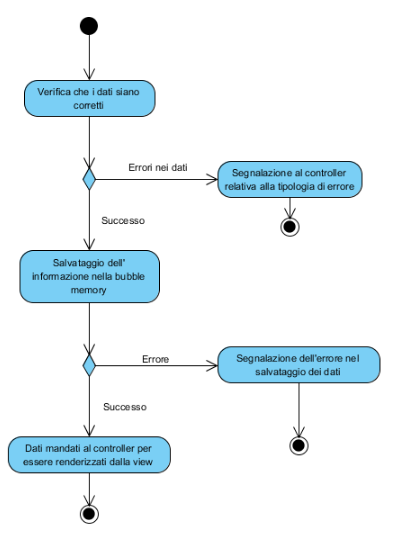
\includegraphics[width=10cm]{../../documenti/SpecificaTecnica/diagrammi_img/attivita/addelementtodolist.png}
	\caption{Diagramma di attività - Aggiunta elemento alla To-do list}
\end{figure}

\begin{figure}[H]
	\centering
	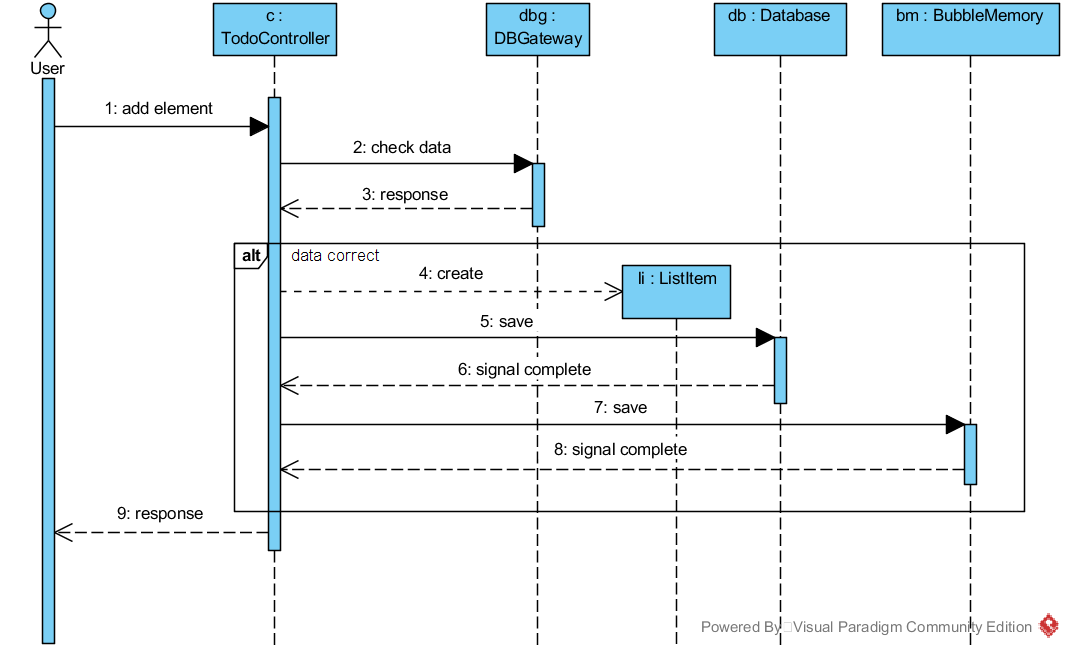
\includegraphics[width=14cm]{diagrammi_img/sequenza/todo_aggiungi_elemento.png}
	\caption{Diagramma di sequenza - Aggiunta elemento alla To-do list}
\end{figure}
Dopo una verifica preliminare della loro correttezza, i dati vengono salvati nella bubble memory e ritornati al controller che li inoltra alla view, da cui saranno renderizzati.
La procedura è analoga anche nel caso in cui si verifichino degli errori, che verranno visualizzati nel medesimo modo.


\paragraph{Rimozione elemento dalla To-do list}\mbox{}\\
\nopagebreak
\begin{figure}[H]
	\centering
	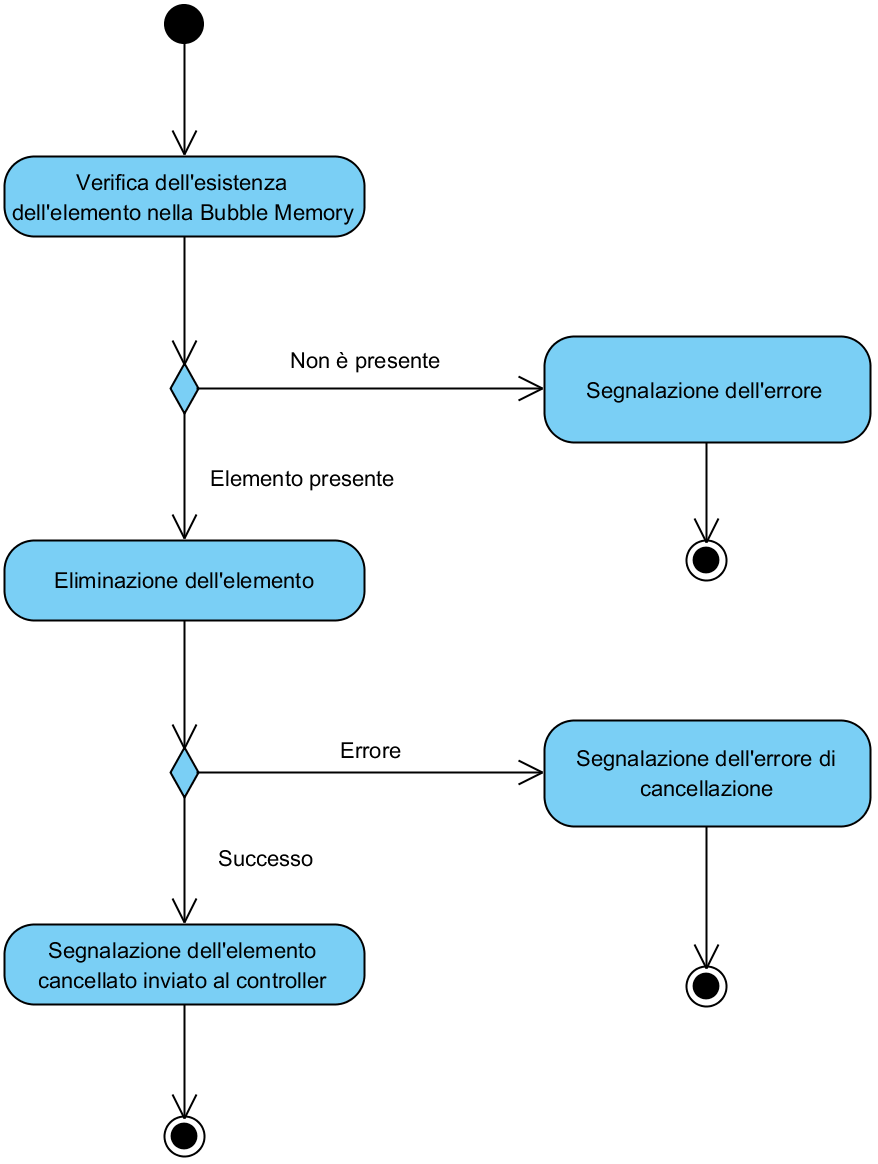
\includegraphics[width=10cm]{../../documenti/SpecificaTecnica/diagrammi_img/attivita/removeelementtodolist.png}
	\caption{Diagramma di attività - Rimozione elemento dalla To-do list}
\end{figure}

\begin{figure}[H]
	\centering
	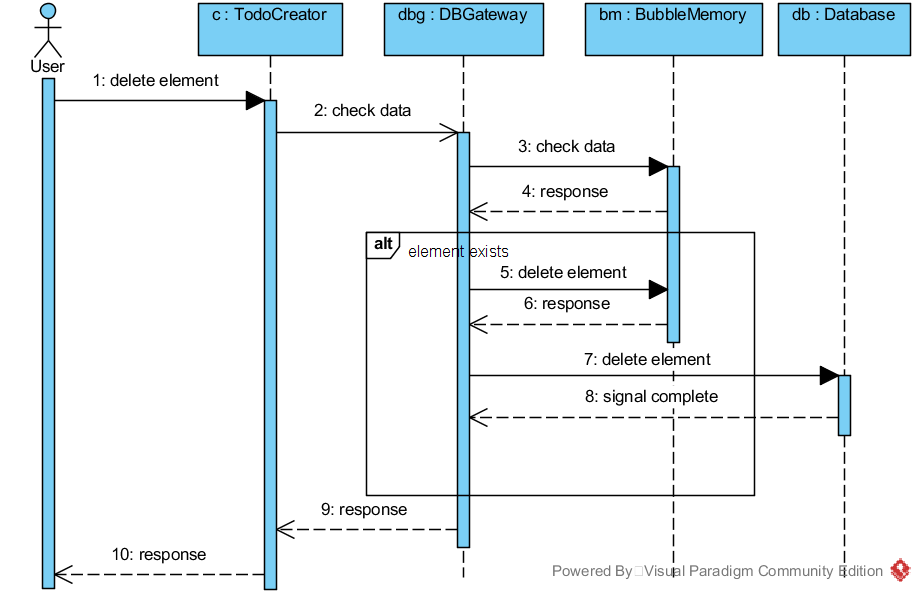
\includegraphics[width=14cm]{../../documenti/SpecificaTecnica/diagrammi_img/sequenza/todo_rimuovi_elemento.png}
	\caption{Diagramma di sequenza - Rimozione elemento dalla To-do list}
\end{figure}
Il procedimento è del tutto analogo a quello adottato per l'aggiunta di un elemento alla To-do list. Inizialmente viene controllato se all'interno della bubble memory è presente l'elemento che si intende eliminare: 
\begin{itemize}
	\item se è presente si procede all'eliminazione;
	\item se non è presente viene effettuata una segnalazione tramite valore di ritorno.
\end{itemize}
Una volta effettuata la rimozione dell'elemento viene ritornato al controller:
\begin{itemize}
	\item lo stesso elemento appena rimosso se l'operazione va a buon fine;
	\item un messaggio di errore altrimenti.
\end{itemize}
Il controller si occupa poi di inoltrare questi messaggi alla view affinché possano essere renderizzati e visualizzati così dall'utente.

\paragraph{Aggiunta notifica statica}\mbox{}\\
\nopagebreak
\begin{figure}[H]
	\centering
	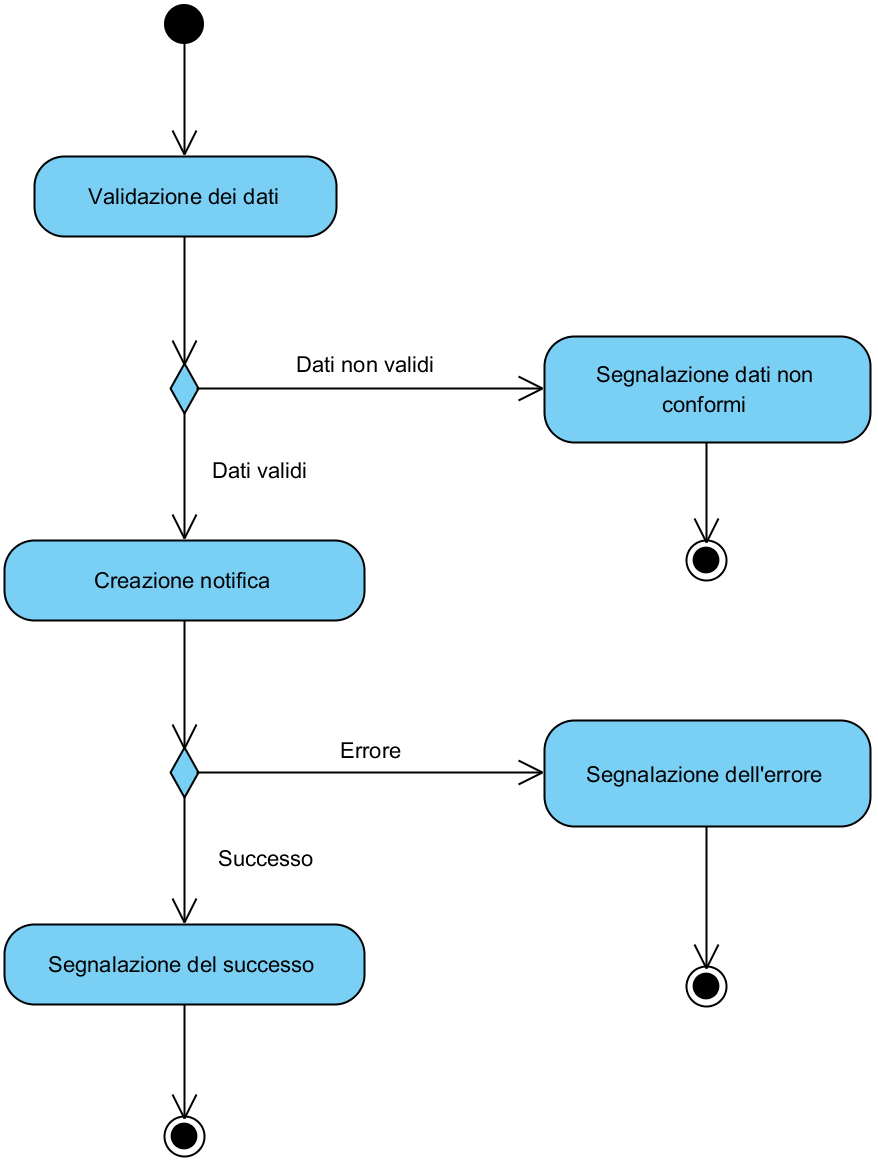
\includegraphics[width=10cm]{../../documenti/SpecificaTecnica/diagrammi_img/attivita/addstaticnotification.png}
	\caption{Diagramma di attività - Aggiunta notifica statica}
\end{figure}

\begin{figure}[H]
	\centering
	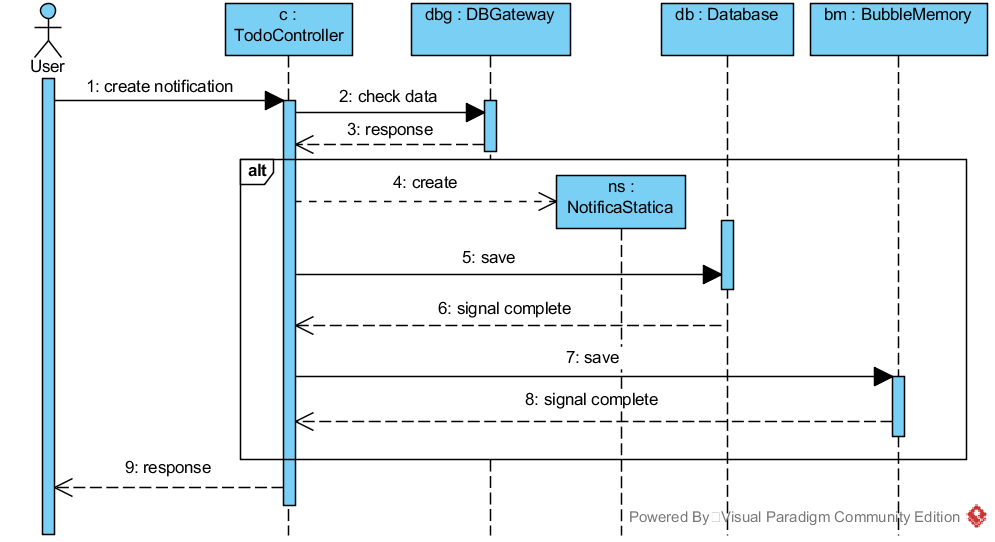
\includegraphics[width=14cm]{../../documenti/SpecificaTecnica/diagrammi_img/sequenza/todo_aggiungi_notifica.png}
	\caption{Diagramma di sequenza - Aggiunta notifica statica}
\end{figure}
I dati inviati dal controller vengono validati prima di essere ricevuti dalla GUI. In caso siano presenti errori l'operazione viene interrotta con un messaggio di errore e la notifica non viene creata. Il messaggio di errore viene quindi inviato alla GUI, affinché possa essere renderizzato e mostrato all'utente. Se invece i dati sono conformi, viene creata una notifica statica. Il successo o meno di questa operazione viene segnalata dal model al controller e dal controller alla GUI, cosicché l'utente sia a conoscenza di quanto successo.

\subsubsection{View}

\paragraph{Flusso principale View}\mbox{}\\
\nopagebreak
\begin{figure}[H]
	\centering
	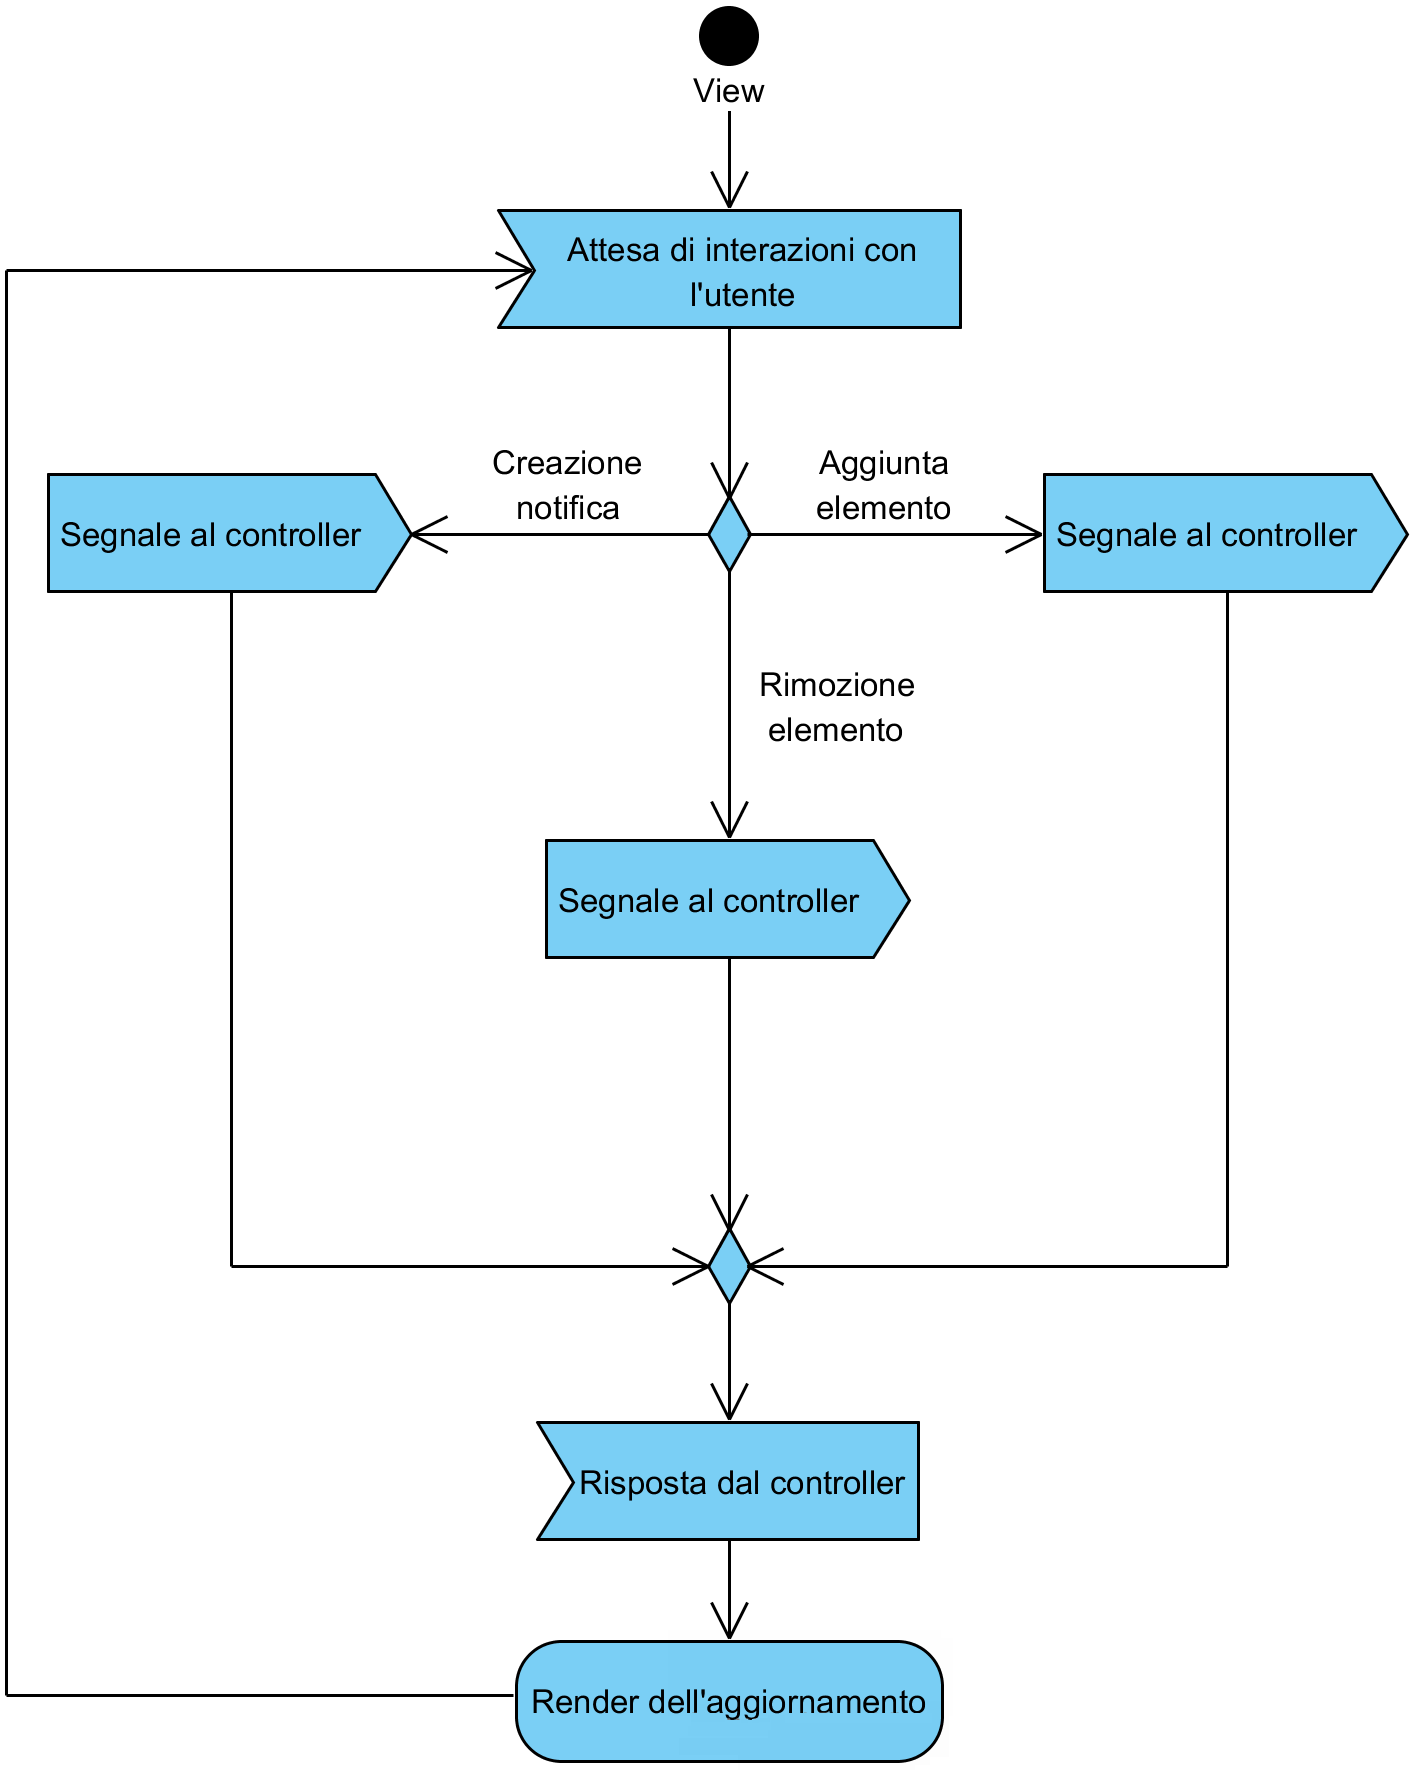
\includegraphics[width=10cm]{../../documenti/SpecificaTecnica/diagrammi_img/attivita/viewmainflow.png}
	\caption{Diagrammi di attività - Flusso principale View}
\end{figure}

Dal punto di vista visuale la bubble apparirà come elenco interattivo composto da una serie di elementi. Selezionando l'apposito pulsante sarà possibile aggiungere o rimuovere un elemento dalla lista. L'aggiunta e la rimozione di elementi della lista comportano un aggiornamento della parte grafica con la conseguente aggiunta o rimozione dell'elemento (rappresentato come testo) dalla lista.\\
Sarà inoltre presente un comando per creare una notifica statica relativa alla lista.\\
L'interazione dell'utente utilizzatore della bubble con l'interfaccia grafica genererà dei segnali che verranno mandati al controller della bubble stessa.

\subsubsection{Controller}

\paragraph{Flusso principale controller}\mbox{}\\
\nopagebreak
\begin{figure}[H]
	\centering
	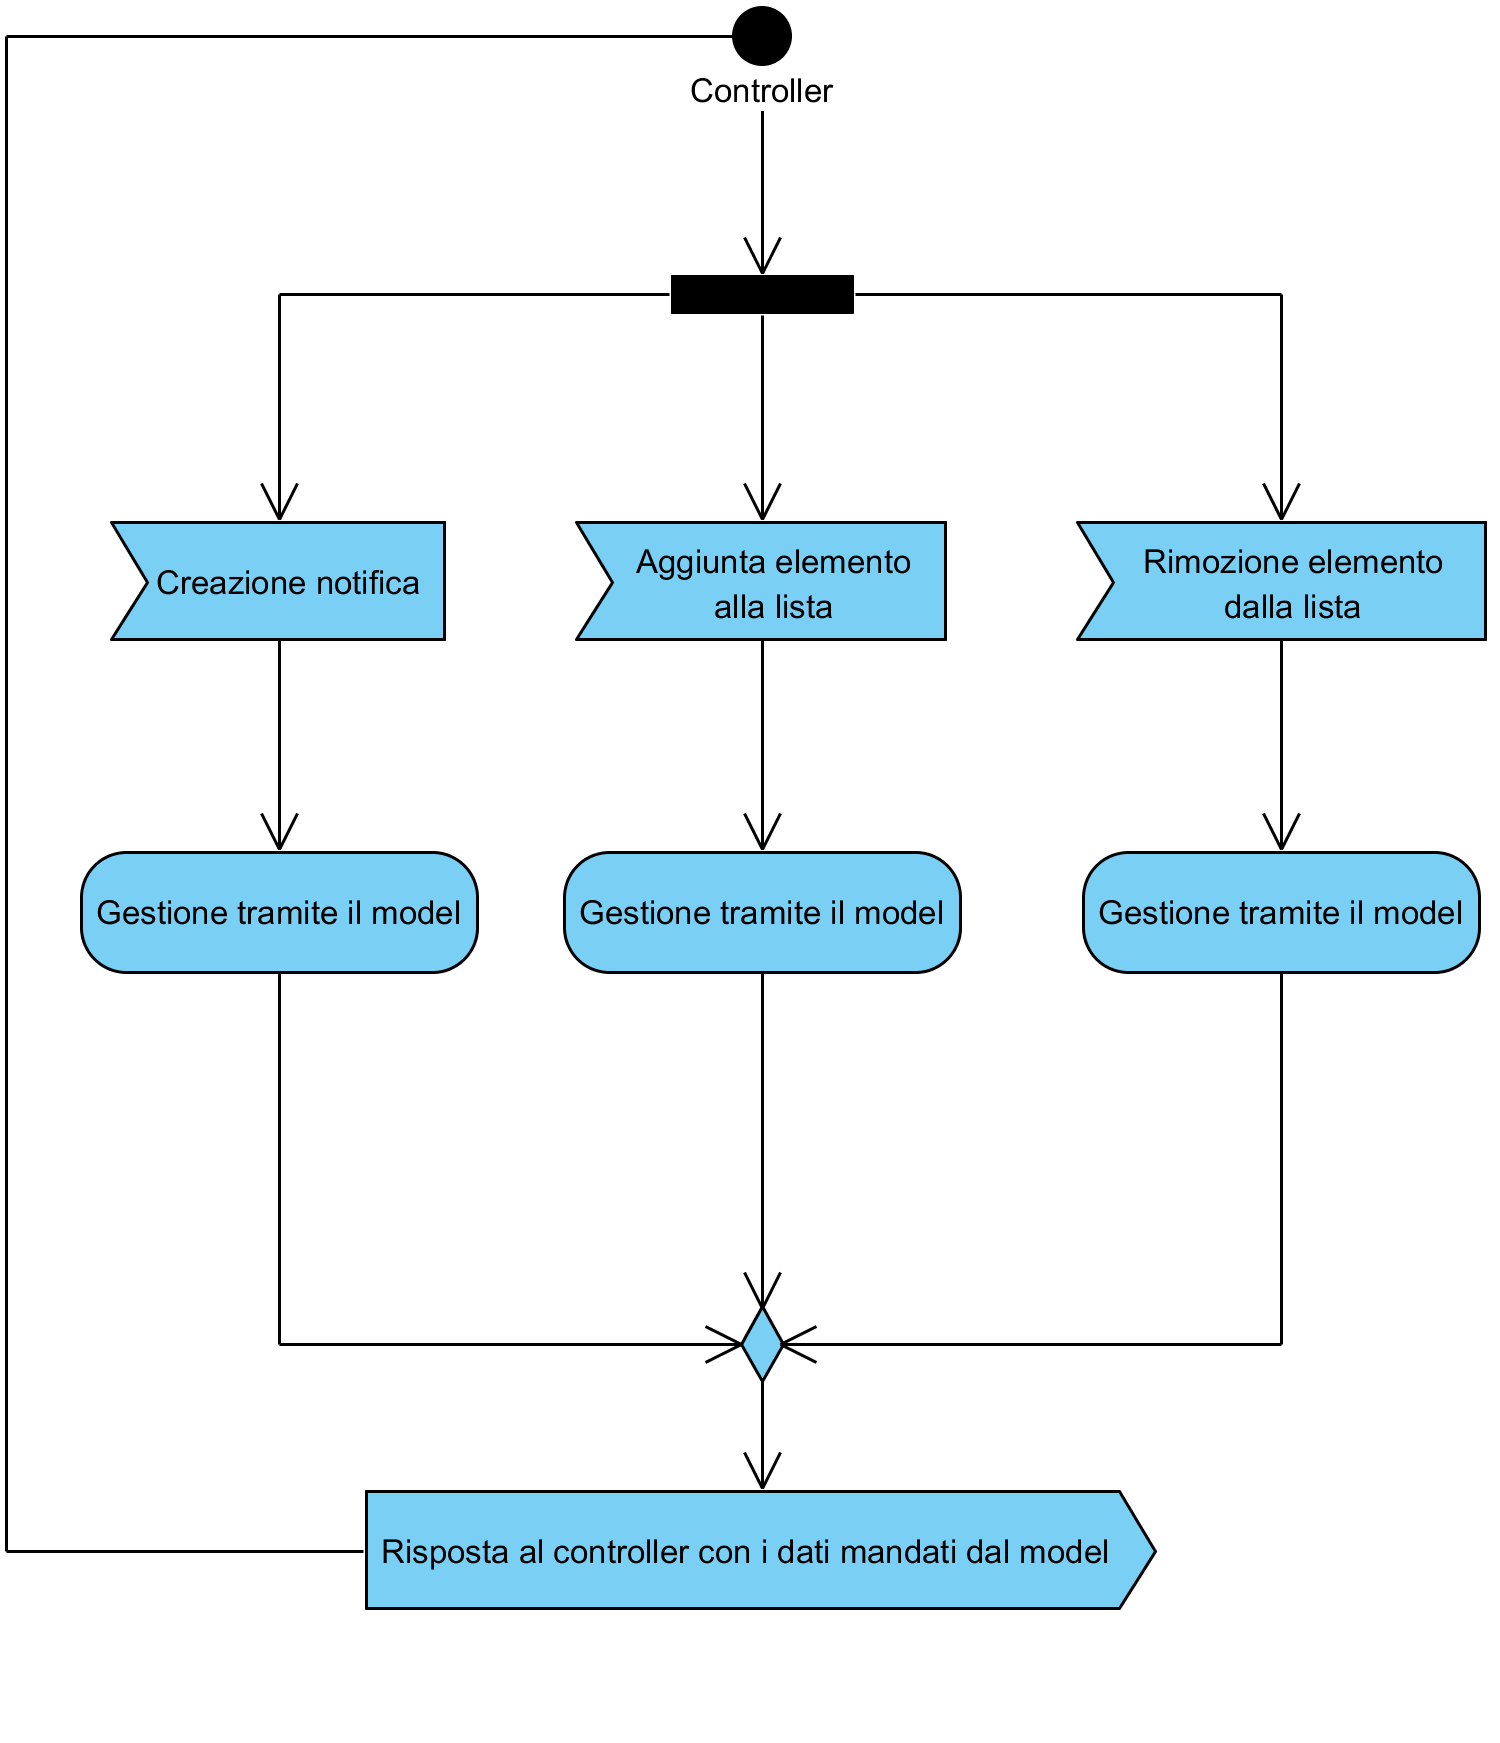
\includegraphics[width=10cm]{../../documenti/SpecificaTecnica/diagrammi_img/attivita/controllermainflow.png}
	\caption{Diagramma di attività - Flusso principale controller}
\end{figure}


Il controller sarà una componente software incaricata di ascoltare e di attendere i segnali generati dall'interfaccia grafica e dalla parte di business logic dell'applicativo, collegandone le funzionalità secondo quanto specificato nei requisiti. 

\subsection{Bubble \& eat}
Nello scenario descritto dalla demo, tramite il framework e le bubble da esso prodotte sarà possibile per gli attori interagire con il sistema nei seguenti modi, suddivisi per attore che li compie.

\subsubsection{\Customer{}}

\paragraph{Inserimento dati personali}\mbox{}\\
\nopagebreak
\begin{figure}[H]
	\centering
	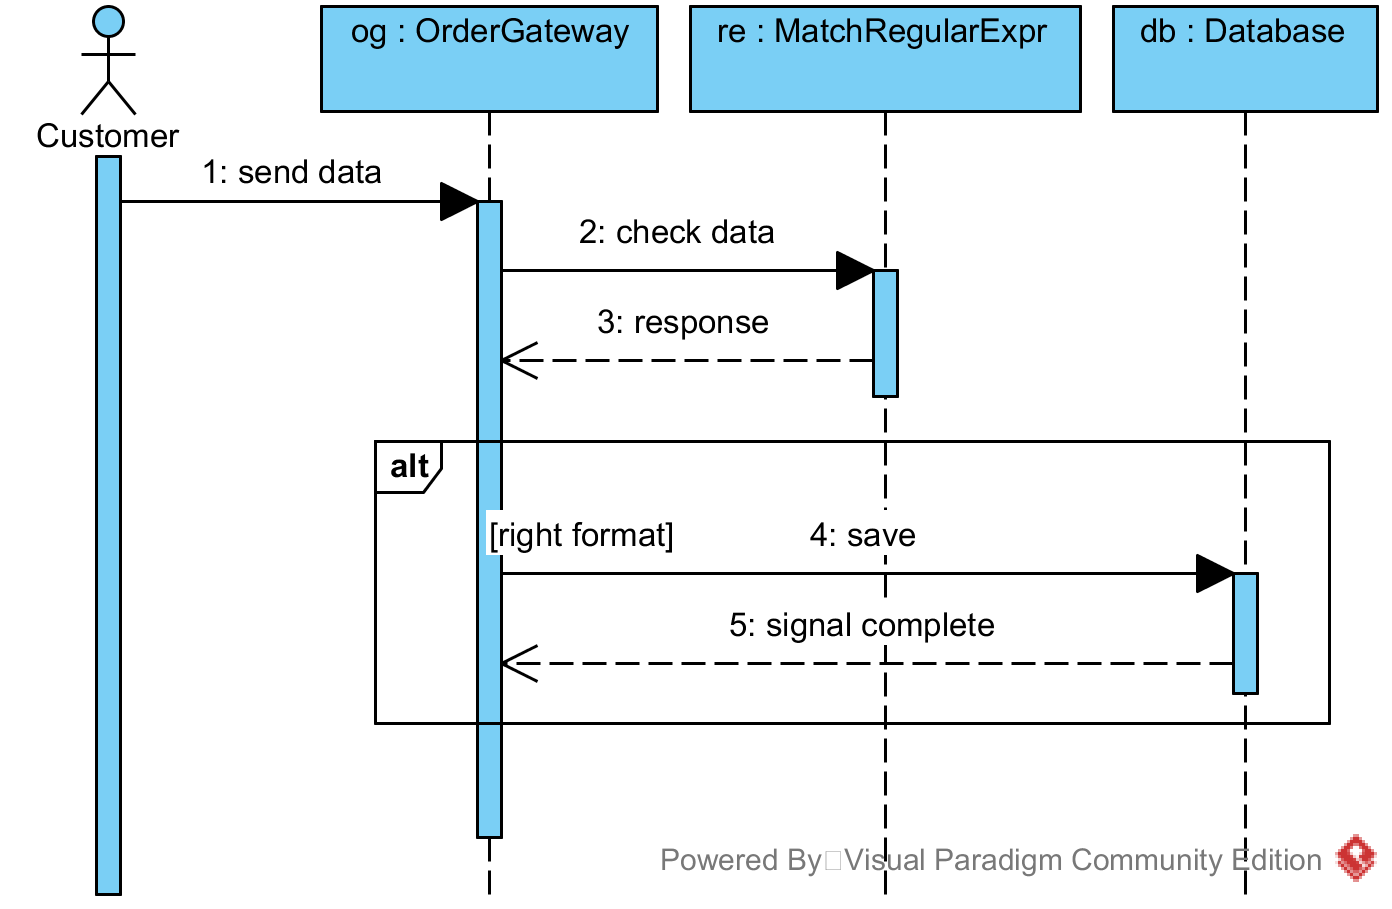
\includegraphics[width=14cm]{diagrammi_img/sequenza/cliente_inserisci_informazioni.png}
	\caption{Diagramma di sequenza - Inserimento dati personali}
\end{figure}
Il \Customer{} inserisce le proprie informazioni e le invia. I dati vengono ricevuti dall'Order\-Gateway, che li verifica tramite MatchRegularExpr e li salva nel database se rispettano il formato prefissato, altrimenti ritorna un messaggio di errore all'utente.


\paragraph{Lettura dal menu}\mbox{}\\
\nopagebreak
\begin{figure}[H]
	\centering
	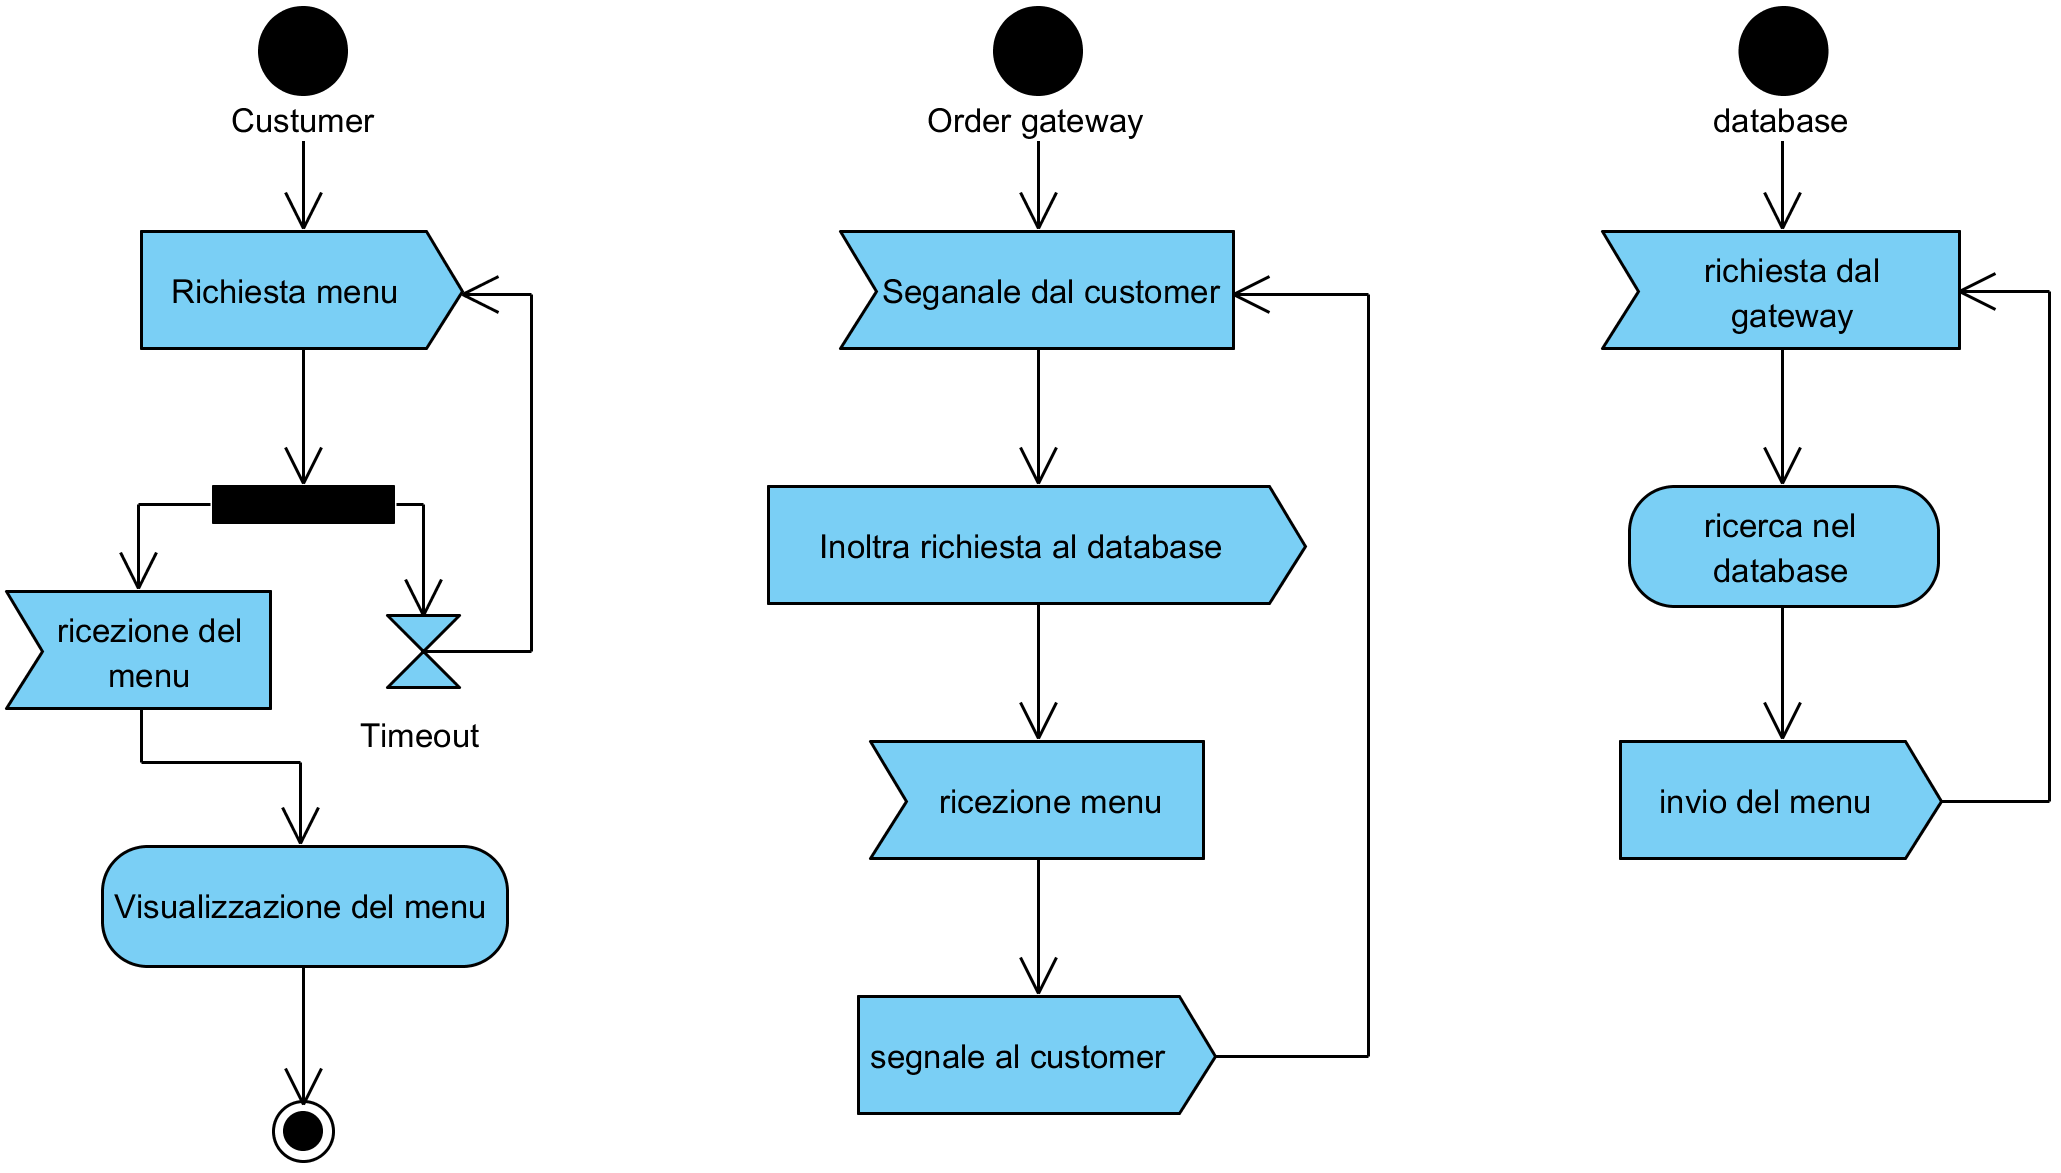
\includegraphics[width=14cm]{diagrammi_img/attivita/costumer_get_menu.png}
	\caption{Diagramma di attività - Lettura dal menu}
\end{figure}

\begin{figure}[H]
	\centering
	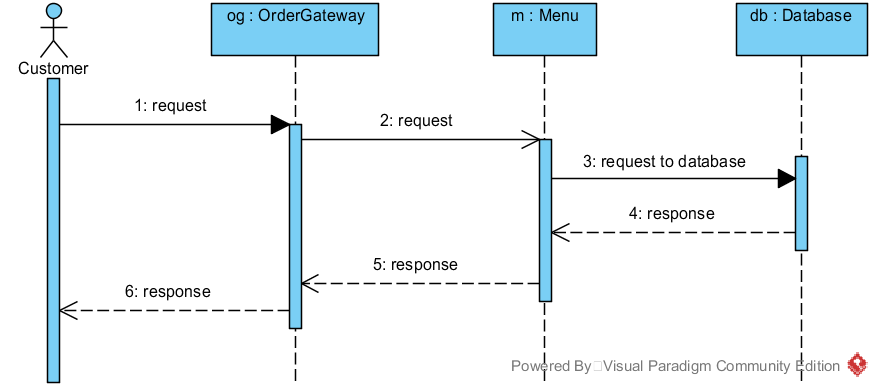
\includegraphics[width=14cm]{../../documenti/SpecificaTecnica/diagrammi_img/sequenza/client_visualizza_menu.png}
	\caption{Diagramma di sequenza - Lettura dal menu}
\end{figure}
Il \Customer{} invia la richiesta di visualizzare il menu, la richiesta viene ricevuta dall'Order\-Gateway ed è inoltrata al database che risponde fornendo il menu, il quale viene inviato poi al \Customer{}.


\paragraph{Fai ordinazione}\mbox{}\\
\nopagebreak
\begin{figure}[H]
	\centering
	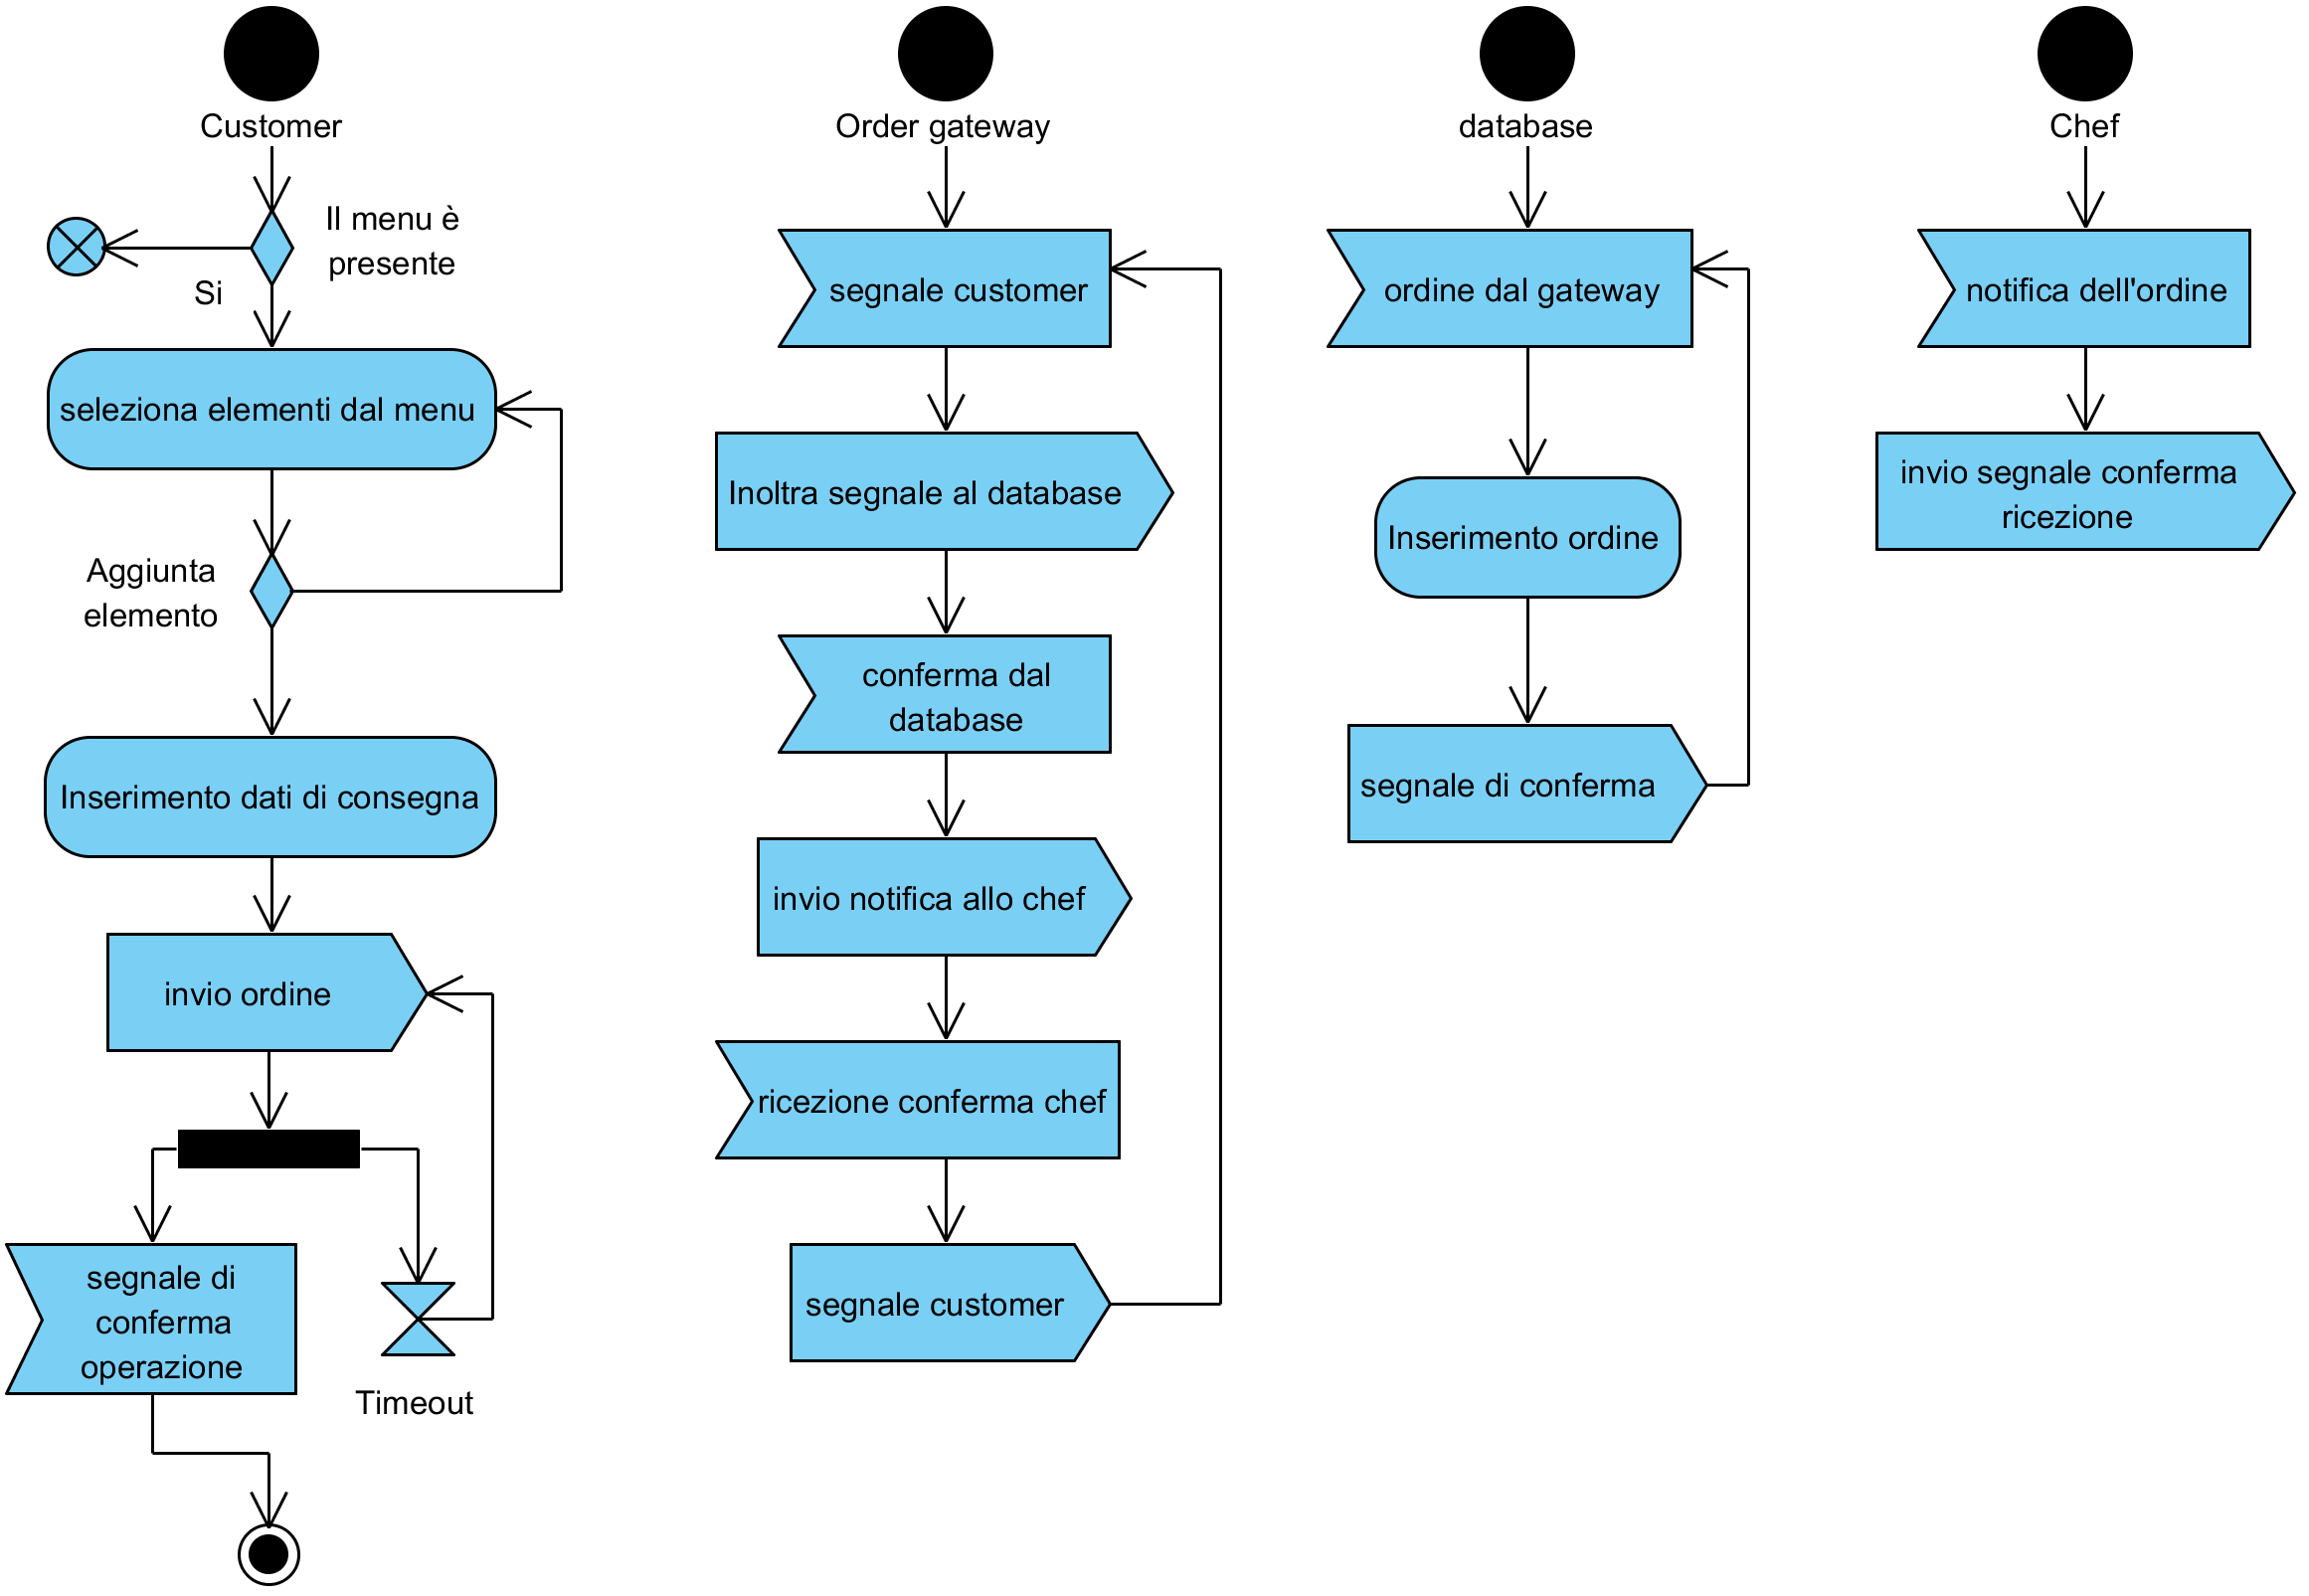
\includegraphics[width=14cm]{diagrammi_img/attivita/customer_ordinazione.png}
	\caption{Diagramma di attività - Fai ordinazione}
\end{figure}

\begin{figure}[H]
	\centering
	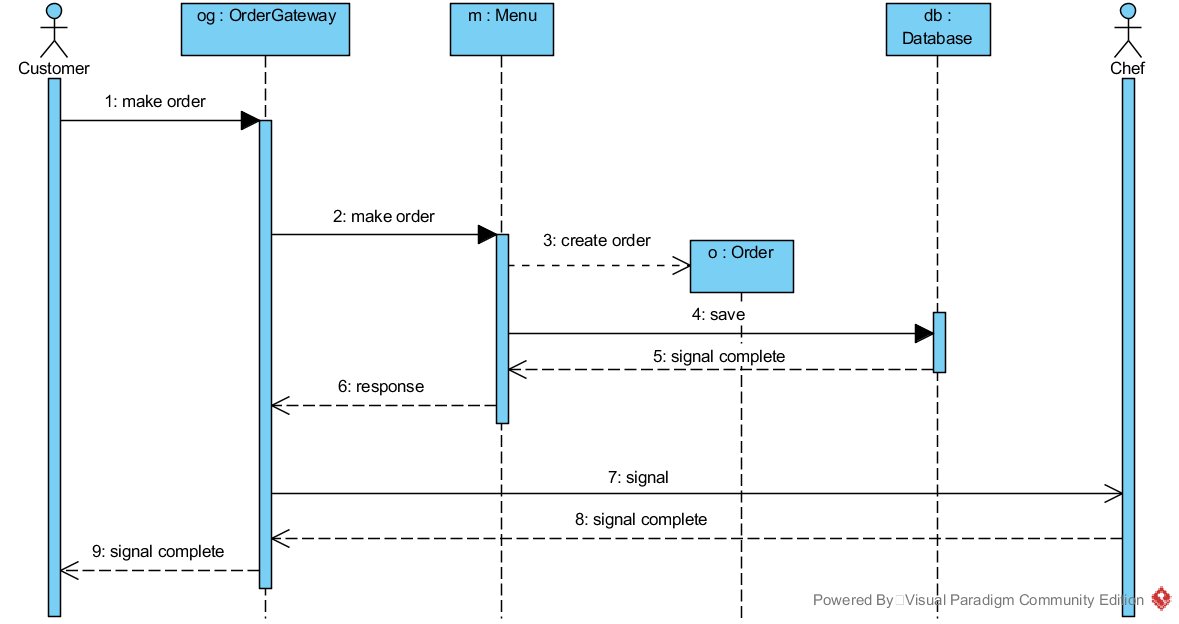
\includegraphics[width=14cm]{../../documenti/SpecificaTecnica/diagrammi_img/sequenza/cliente_fai_ordinazione.png}
	\caption{Diagramma di sequenza - Fai ordinazione}
\end{figure}
Selezionate le pietanze l'ordine è inviato all'Order\-Gateway, il quale salva nel database un'approssimazione delle risorse che verranno consumate nella preparazione; fatto questo l'ordinazione viene inviata allo \Chef{} che provvederà a preparare il piatto.

\subsubsection{\Chef{}}

\paragraph{Conferma completata la preparazione del piatto}\mbox{}\\
\nopagebreak
\begin{figure}[H]
	\centering
	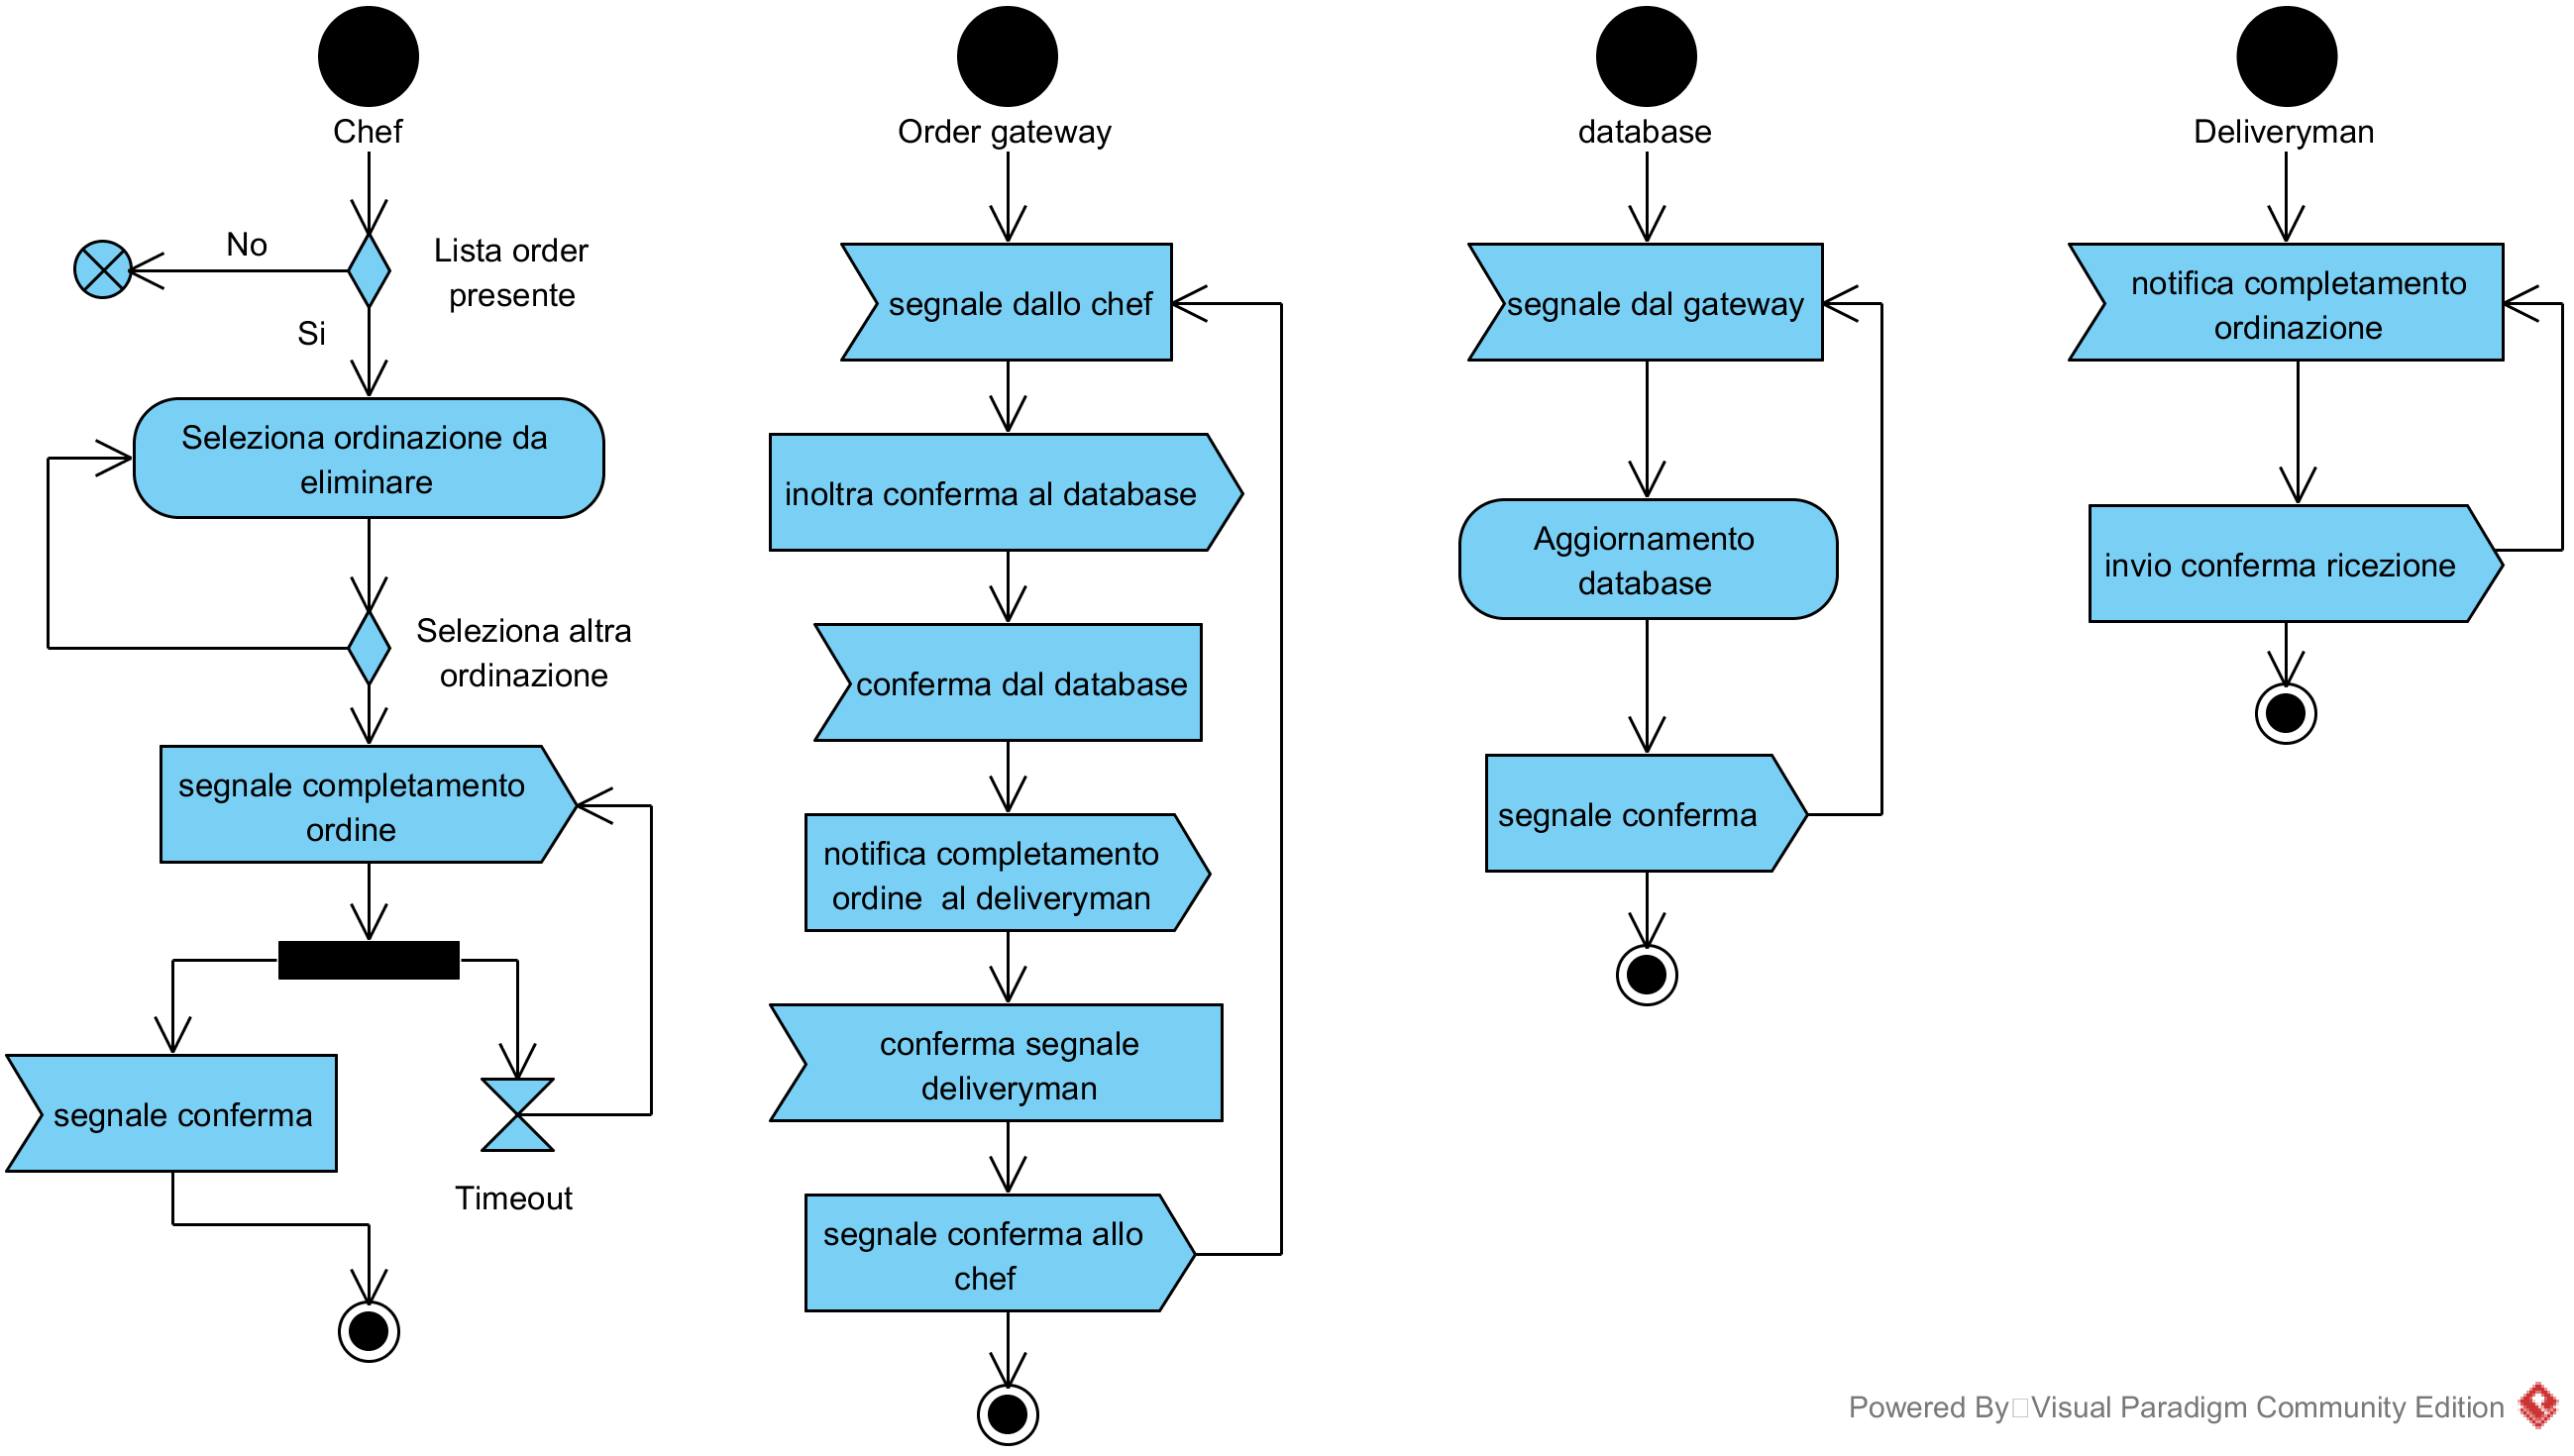
\includegraphics[width=14cm]{diagrammi_img/attivita/chef_comlete_order.png}
\caption{Diagramma di attività - Conferma completata la preparazione del piatto}
\end{figure}

\begin{figure}[H]
	\centering
	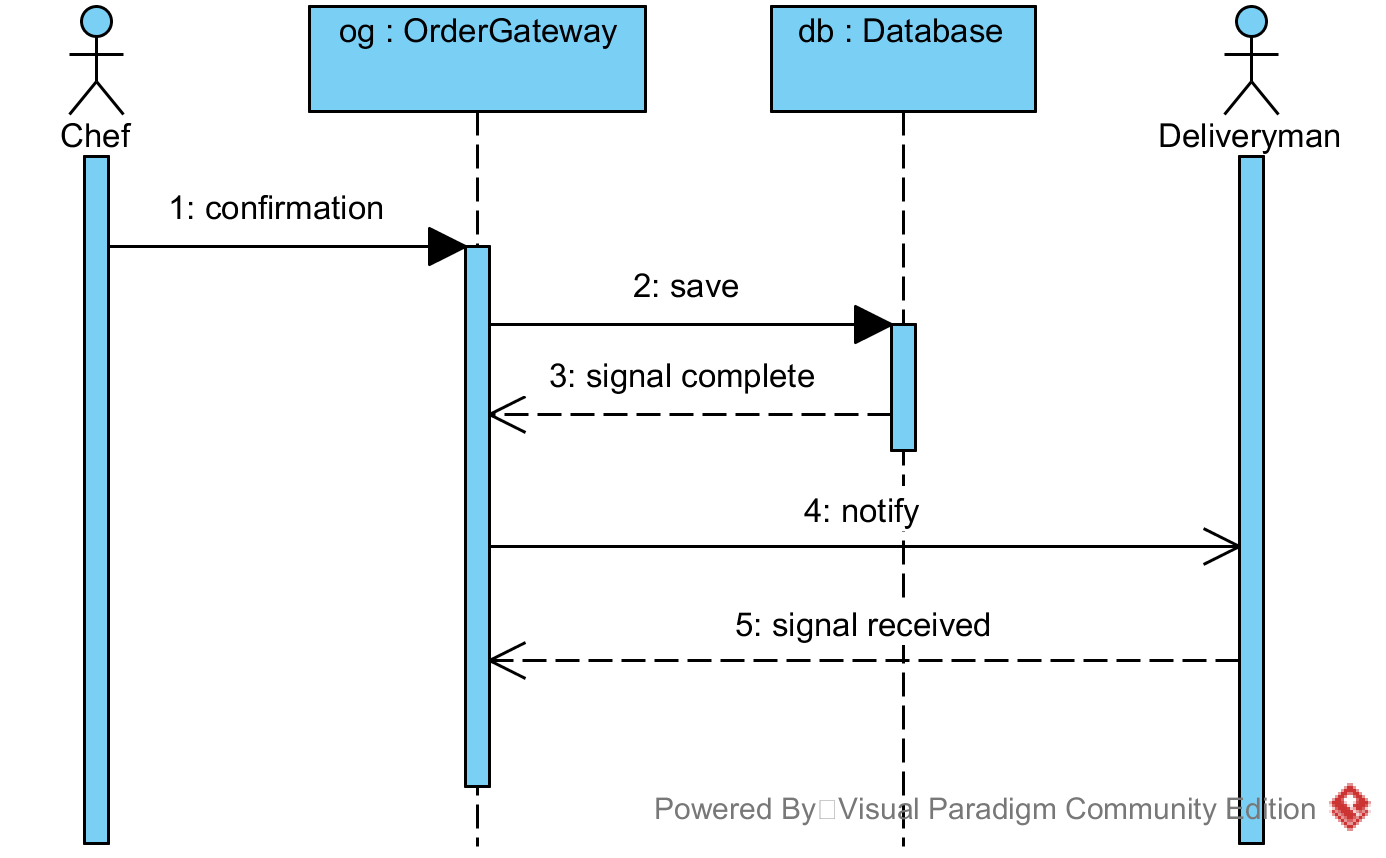
\includegraphics[width=14cm]{diagrammi_img/sequenza/cuoco_piatto_pronto.png}
	\caption{Diagramma di sequenza - Conferma completata la preparazione del piatto}
\end{figure}
Completata la preparazione della pietanza, lo \Chef{} segnala l'avvenuta preparazione all'Order\-Gateway. L'Order\-Gateway provvede a registrare l'ordine pronto nel Database, il quale conferma il salvataggio o ritorna un errore. Al completamento dell'operazione in modo corretto, l'Order\-Gateway invia un segnale di conferma per lo \Chef{} e uno di notifica per il \Deliveryman{}.

\subsubsection{\Deliveryman{}}

\paragraph{Seleziona consegna}\mbox{}\\
\nopagebreak
\begin{figure}[H]
	\centering
	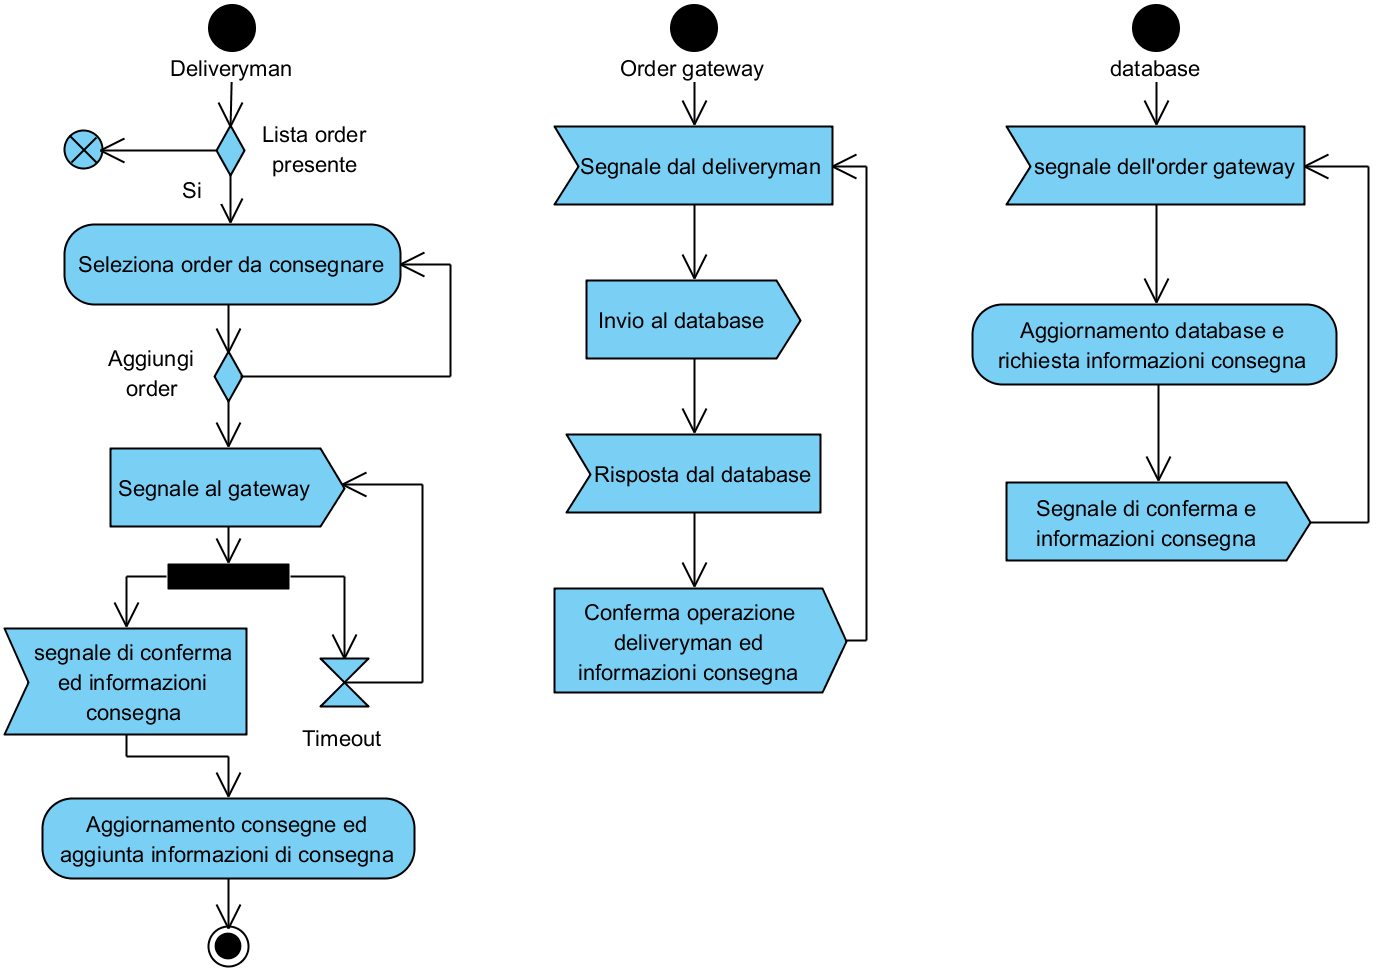
\includegraphics[width=14cm]{diagrammi_img/attivita/deliveryman_seleziona.png}
	\caption{Diagramma di attività - Seleziona consegna}
\end{figure}

\begin{figure}[H]
	\centering
	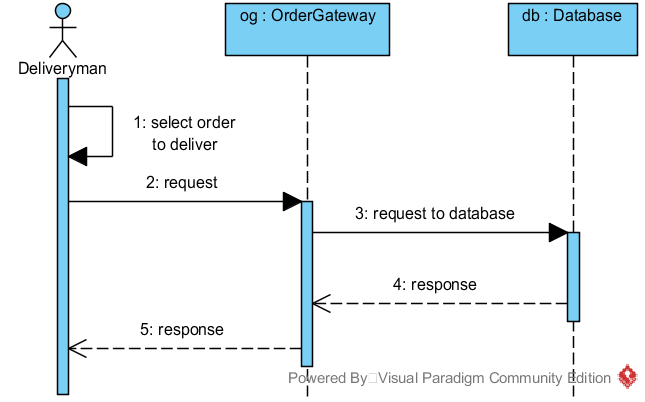
\includegraphics[width=14cm]{../../documenti/SpecificaTecnica/diagrammi_img/sequenza/fattorino_seleziona_consegna.png}
	\caption{Diagramma di sequenza - Seleziona consegna}
\end{figure}

Selezionati gli ordini da consegnare il \Deliveryman{} invia un segnale all'Order\-Gateway, il quale inoltra gli ordini al database; il database quindi aggiorna lo stato degli ordini ricevuti e ricava le informazioni personali degli utenti per la consegna, inviandole come risposta all'Order\-Gateway. A questo punto l'operazione viene confermata e le informazioni di consegna spedite al \Deliveryman{}, il quale può procedere con le consegne.


\paragraph{Segnala la consegna come compiuta}\mbox{}\\
\nopagebreak
\begin{figure}[H]
	\centering
	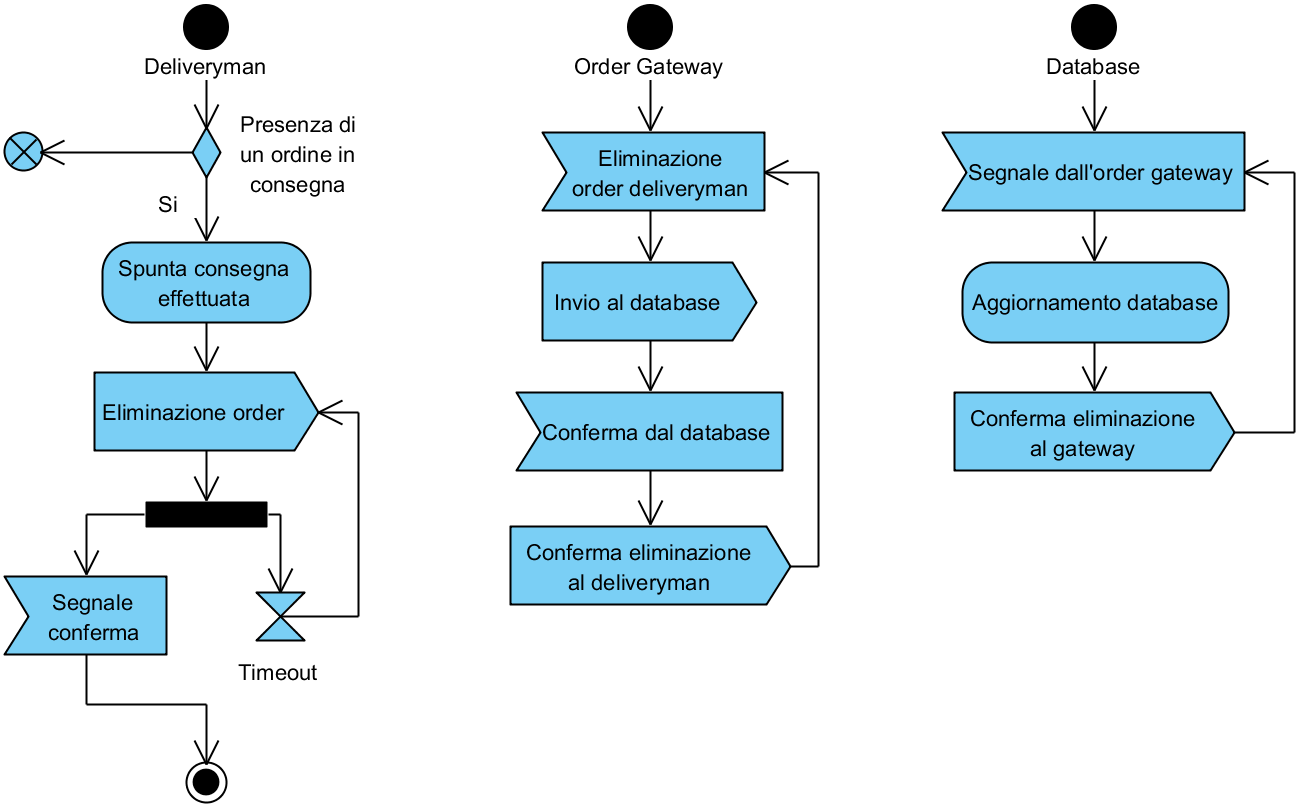
\includegraphics[width=14cm]{diagrammi_img/attivita/deliveryman_consegnato.png}
	\caption{Diagramma di attività - Segnala la consegna come compiuta}
\end{figure}

\begin{figure}[H]
	\centering
	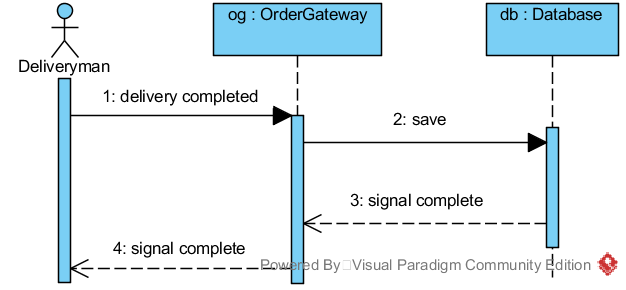
\includegraphics[width=14cm]{../../documenti/SpecificaTecnica/diagrammi_img/sequenza/fattorino_segnala_consegna_completata.png}
	\caption{Diagramma di sequenza - Segnala la consegna come compiuta}
\end{figure}
Una volta completata la consegna il \Deliveryman{} lo segnala all'Order\-Gateway, il quale inoltra l'informazione al database. Vengono quindi salvate le informazioni nel database, il quale ritorna un segnale di conferma, ricevuto dall'Order\-Gateway ed inoltrato al \Deliveryman{}.


\paragraph{Segnala fallimento}\mbox{}\\
\nopagebreak
\begin{figure}[H]
	\centering
	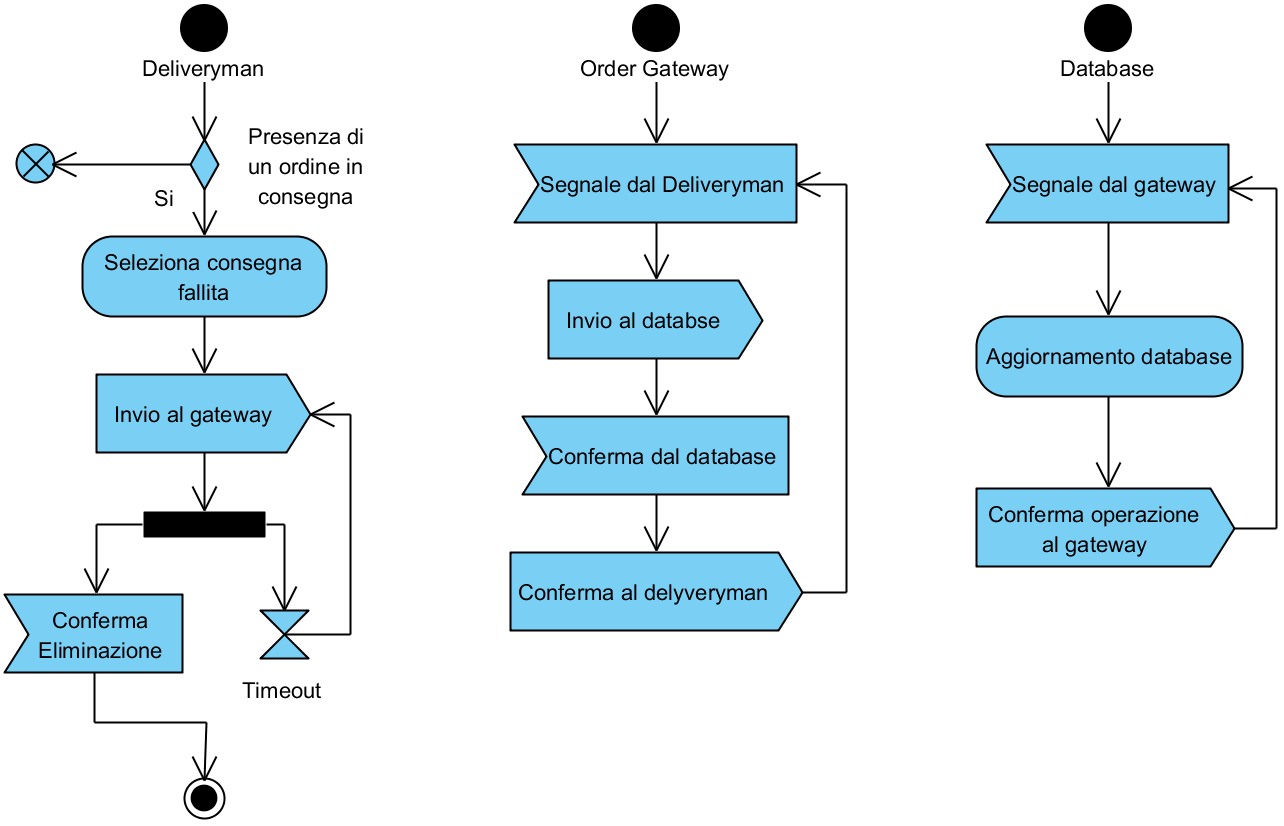
\includegraphics[width=14cm]{diagrammi_img/attivita/delivetyman_fallimento.png}
	\caption{Diagramma di attività - Segnala fallimento}
\end{figure}

\begin{figure}[H]
	\centering
	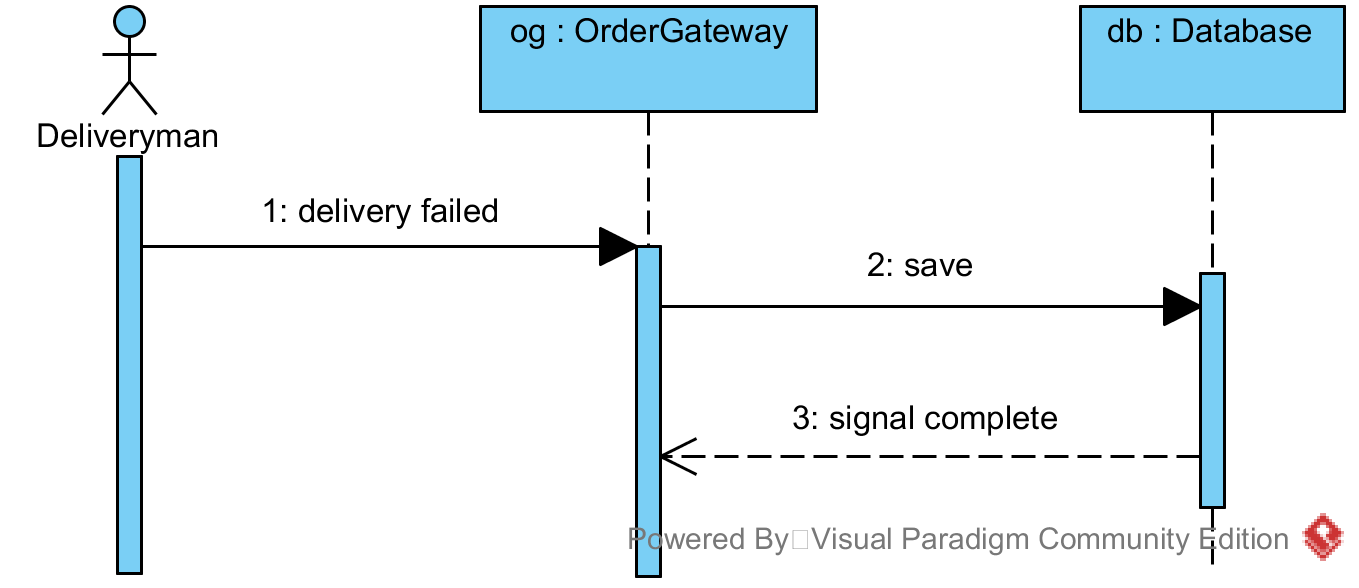
\includegraphics[width=14cm]{../../documenti/SpecificaTecnica/diagrammi_img/sequenza/fattorino_fallimento_consegna.png}
	\caption{Diagramma di sequenza - Segnala fallimento}
\end{figure}
Se la consegna non è andata a buon fine il \Deliveryman{} lo segnala all'Order\-Gateway, il quale inoltra l'informazione al database. Vengono quindi salvate le informazioni nel database, il quale ritorna un segnale di conferma, ricevuto dall'Order\-Gateway ed inoltrato al \Deliveryman{}.

\subsubsection{\Purchasingmanager{}}


\paragraph{Segnala acquistate le scorte}\mbox{}\\
\nopagebreak
\begin{figure}[H]
	\centering
	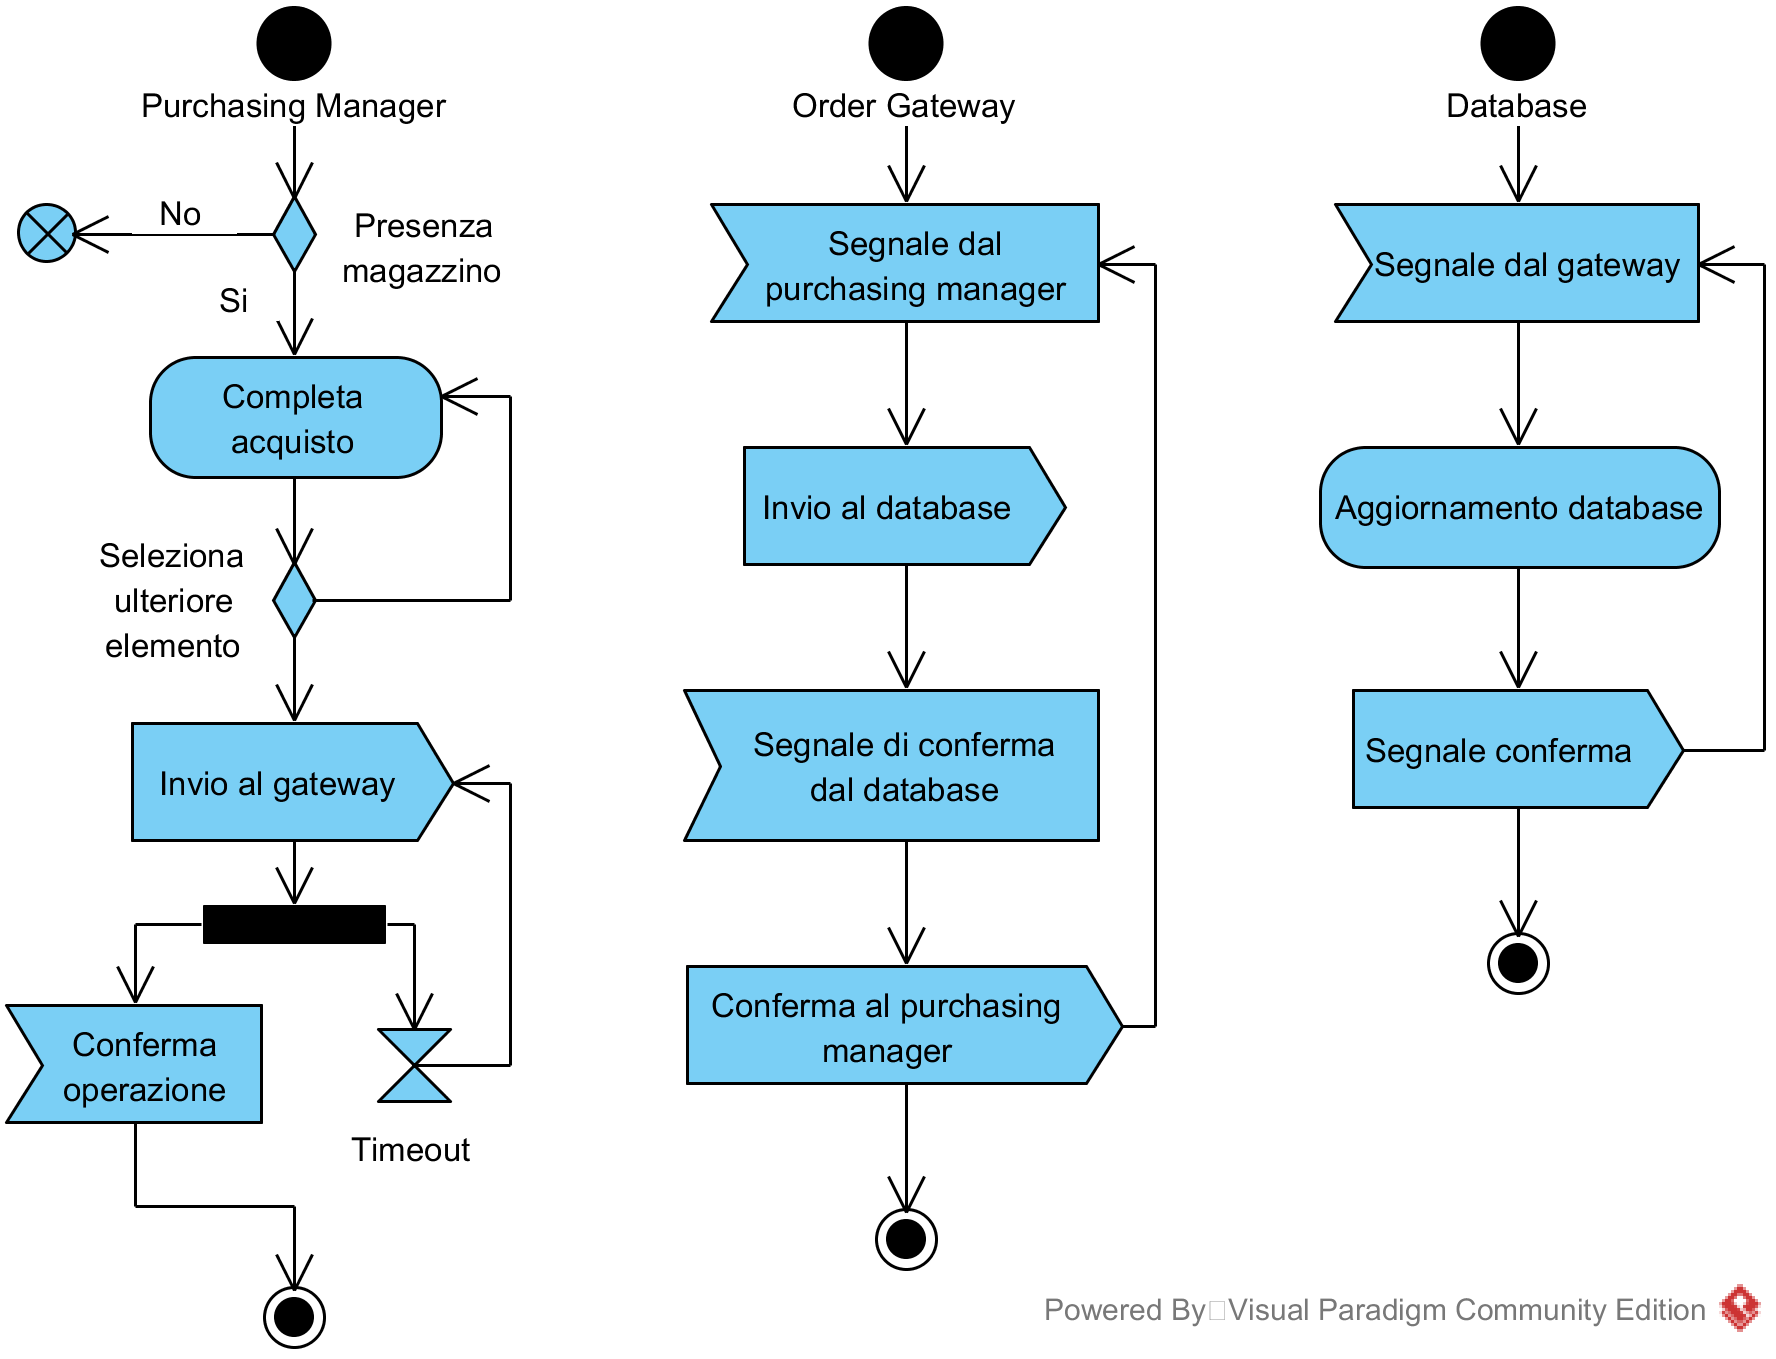
\includegraphics[width=14cm]{diagrammi_img/attivita/responsabile_acquisto.png}
	\caption{Diagramma di attività - Segnala acquistate le scorte}
\end{figure}

\begin{figure}[H]
	\centering
	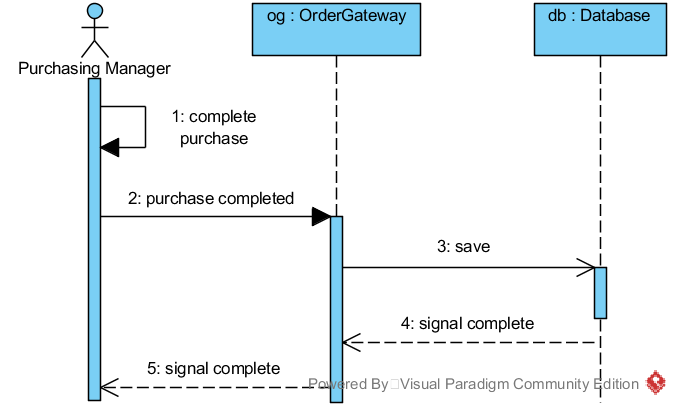
\includegraphics[width=14cm]{../../documenti/SpecificaTecnica/diagrammi_img/sequenza/responsabile_acquisti_segnala_scorte_acquistate.png}
	\caption{Diagramma di sequenza - Segnala acquistate le scorte}
\end{figure}
Il \Purchasingmanager{} segnala l'acquisto delle scorte all'Order\-Gateway. L'Order\-Gateway effettua il salvataggio nel Database dei dati riguardanti le scorte acquistate. Il Database, al completamento dell'operazione, invia un segnale che viene poi riportato dall'Order\-Gateway al \Purchasingmanager{}.

\subsubsection{\Manager{}}

\paragraph{Visualizzazione menu}\mbox{}\\
\nopagebreak
\begin{figure}[H]
	\centering
	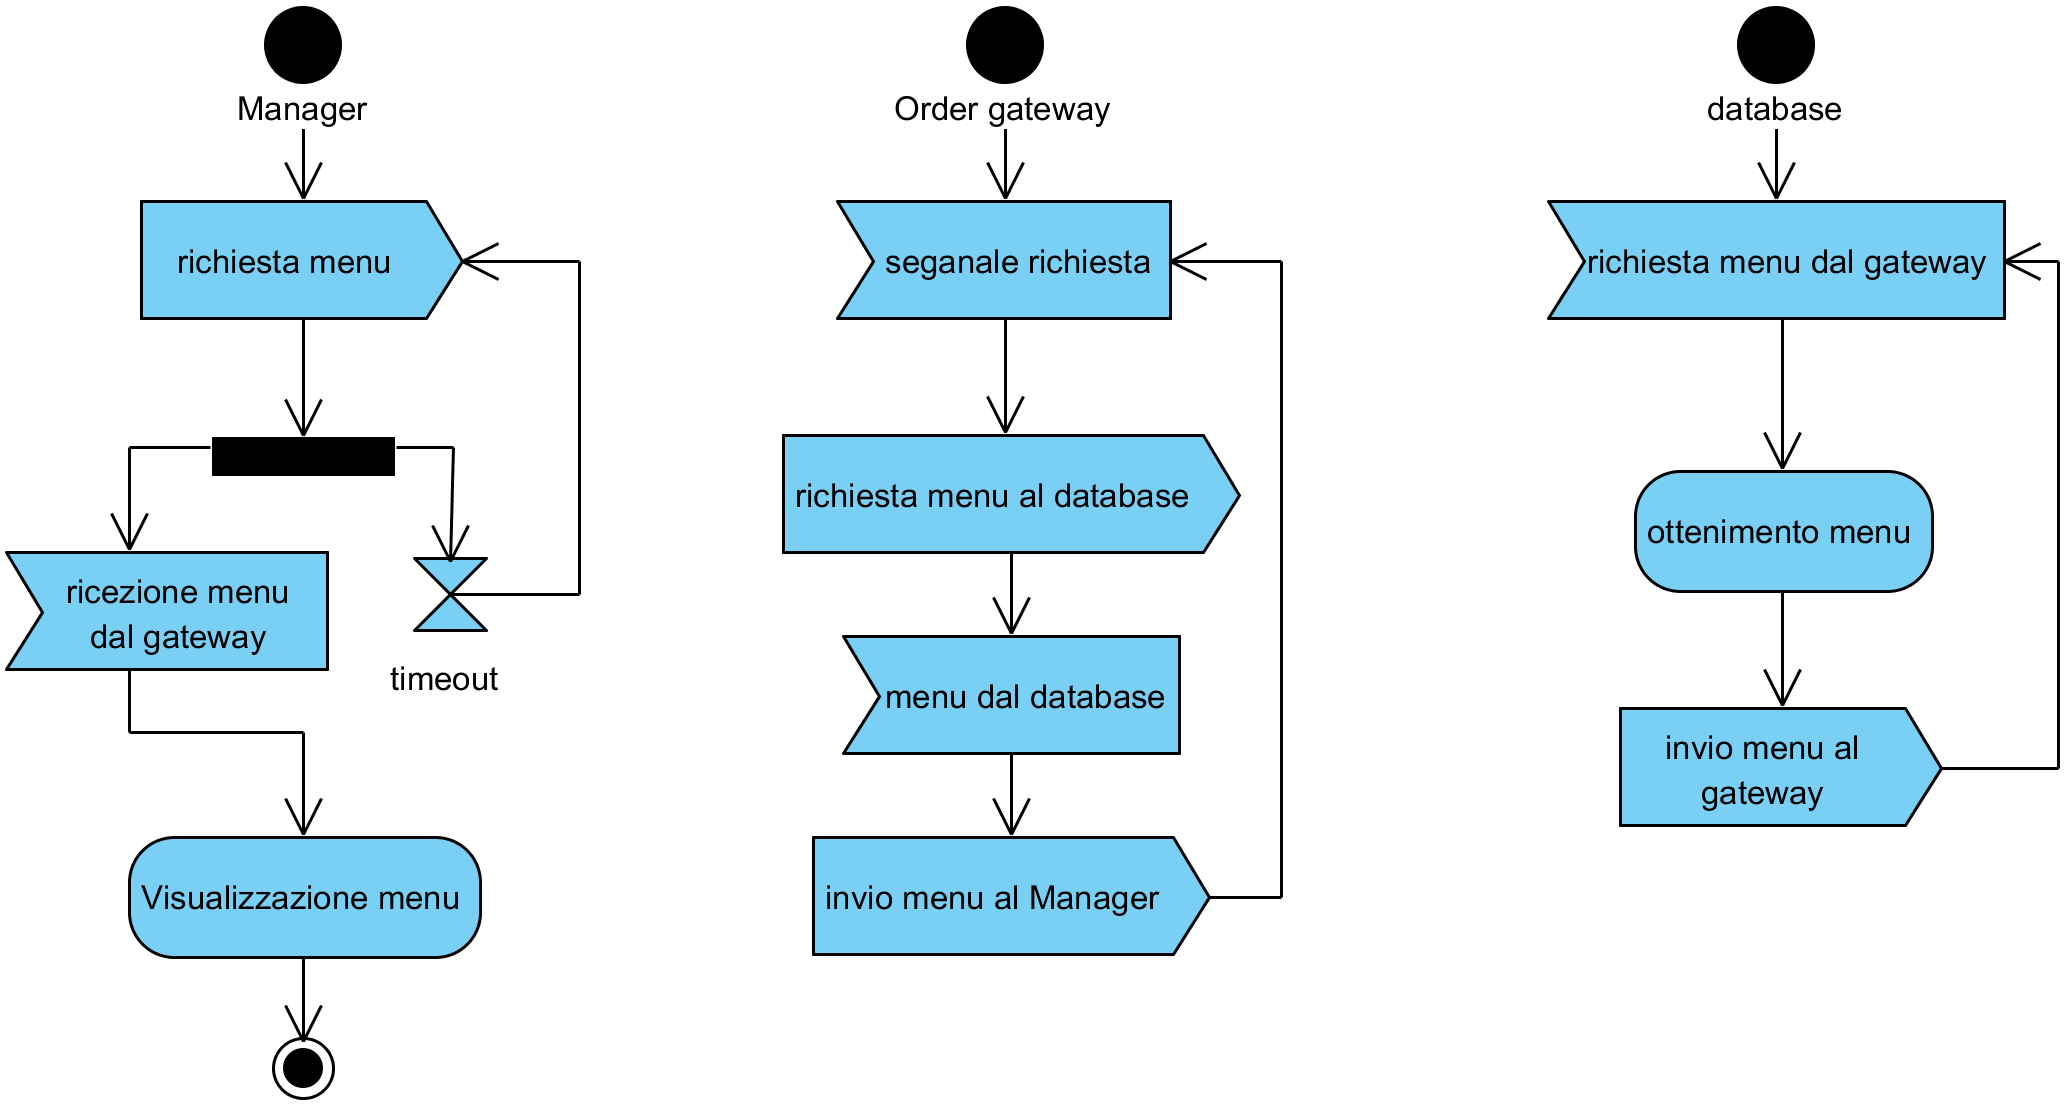
\includegraphics[width=14cm]{diagrammi_img/attivita/manager_get_menu.png}
	\caption{Diagramma di attività - Visualizzazione menu}
\end{figure}

\begin{figure}[H]
	\centering
	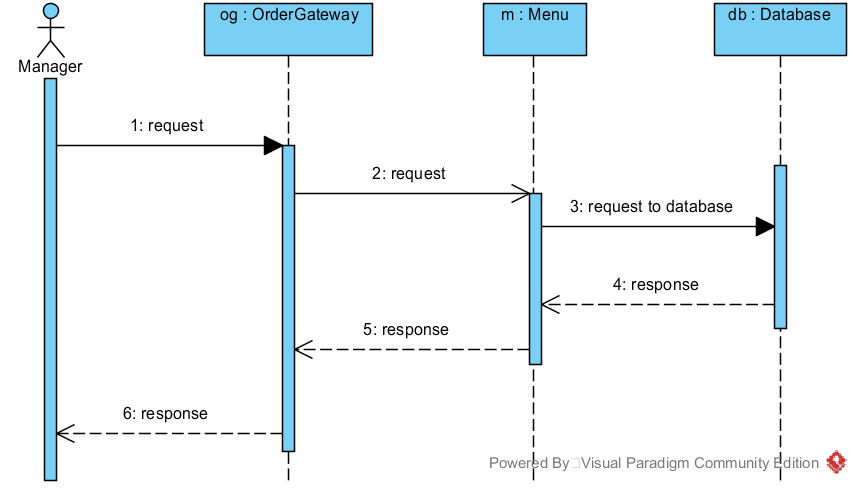
\includegraphics[width=14cm]{../../documenti/SpecificaTecnica/diagrammi_img/sequenza/direttore_visualizza_menu.png}
	\caption{Diagramma di sequenza - Visualizzazione menu}
\end{figure}
Il \Manager{} effettua una richiesta per visualizzare il menu, ricevuta dall'Order\-Gateway ed inoltrata al database, il quale ricerca le informazioni richieste e le ritorna in risposta all'Order\-Gateway. Questo a sua volta le inoltra al \Manager{} che visualizza il menu.

\paragraph{Modifica menu}\mbox{}\\
\nopagebreak
\begin{figure}[H]
	\centering
	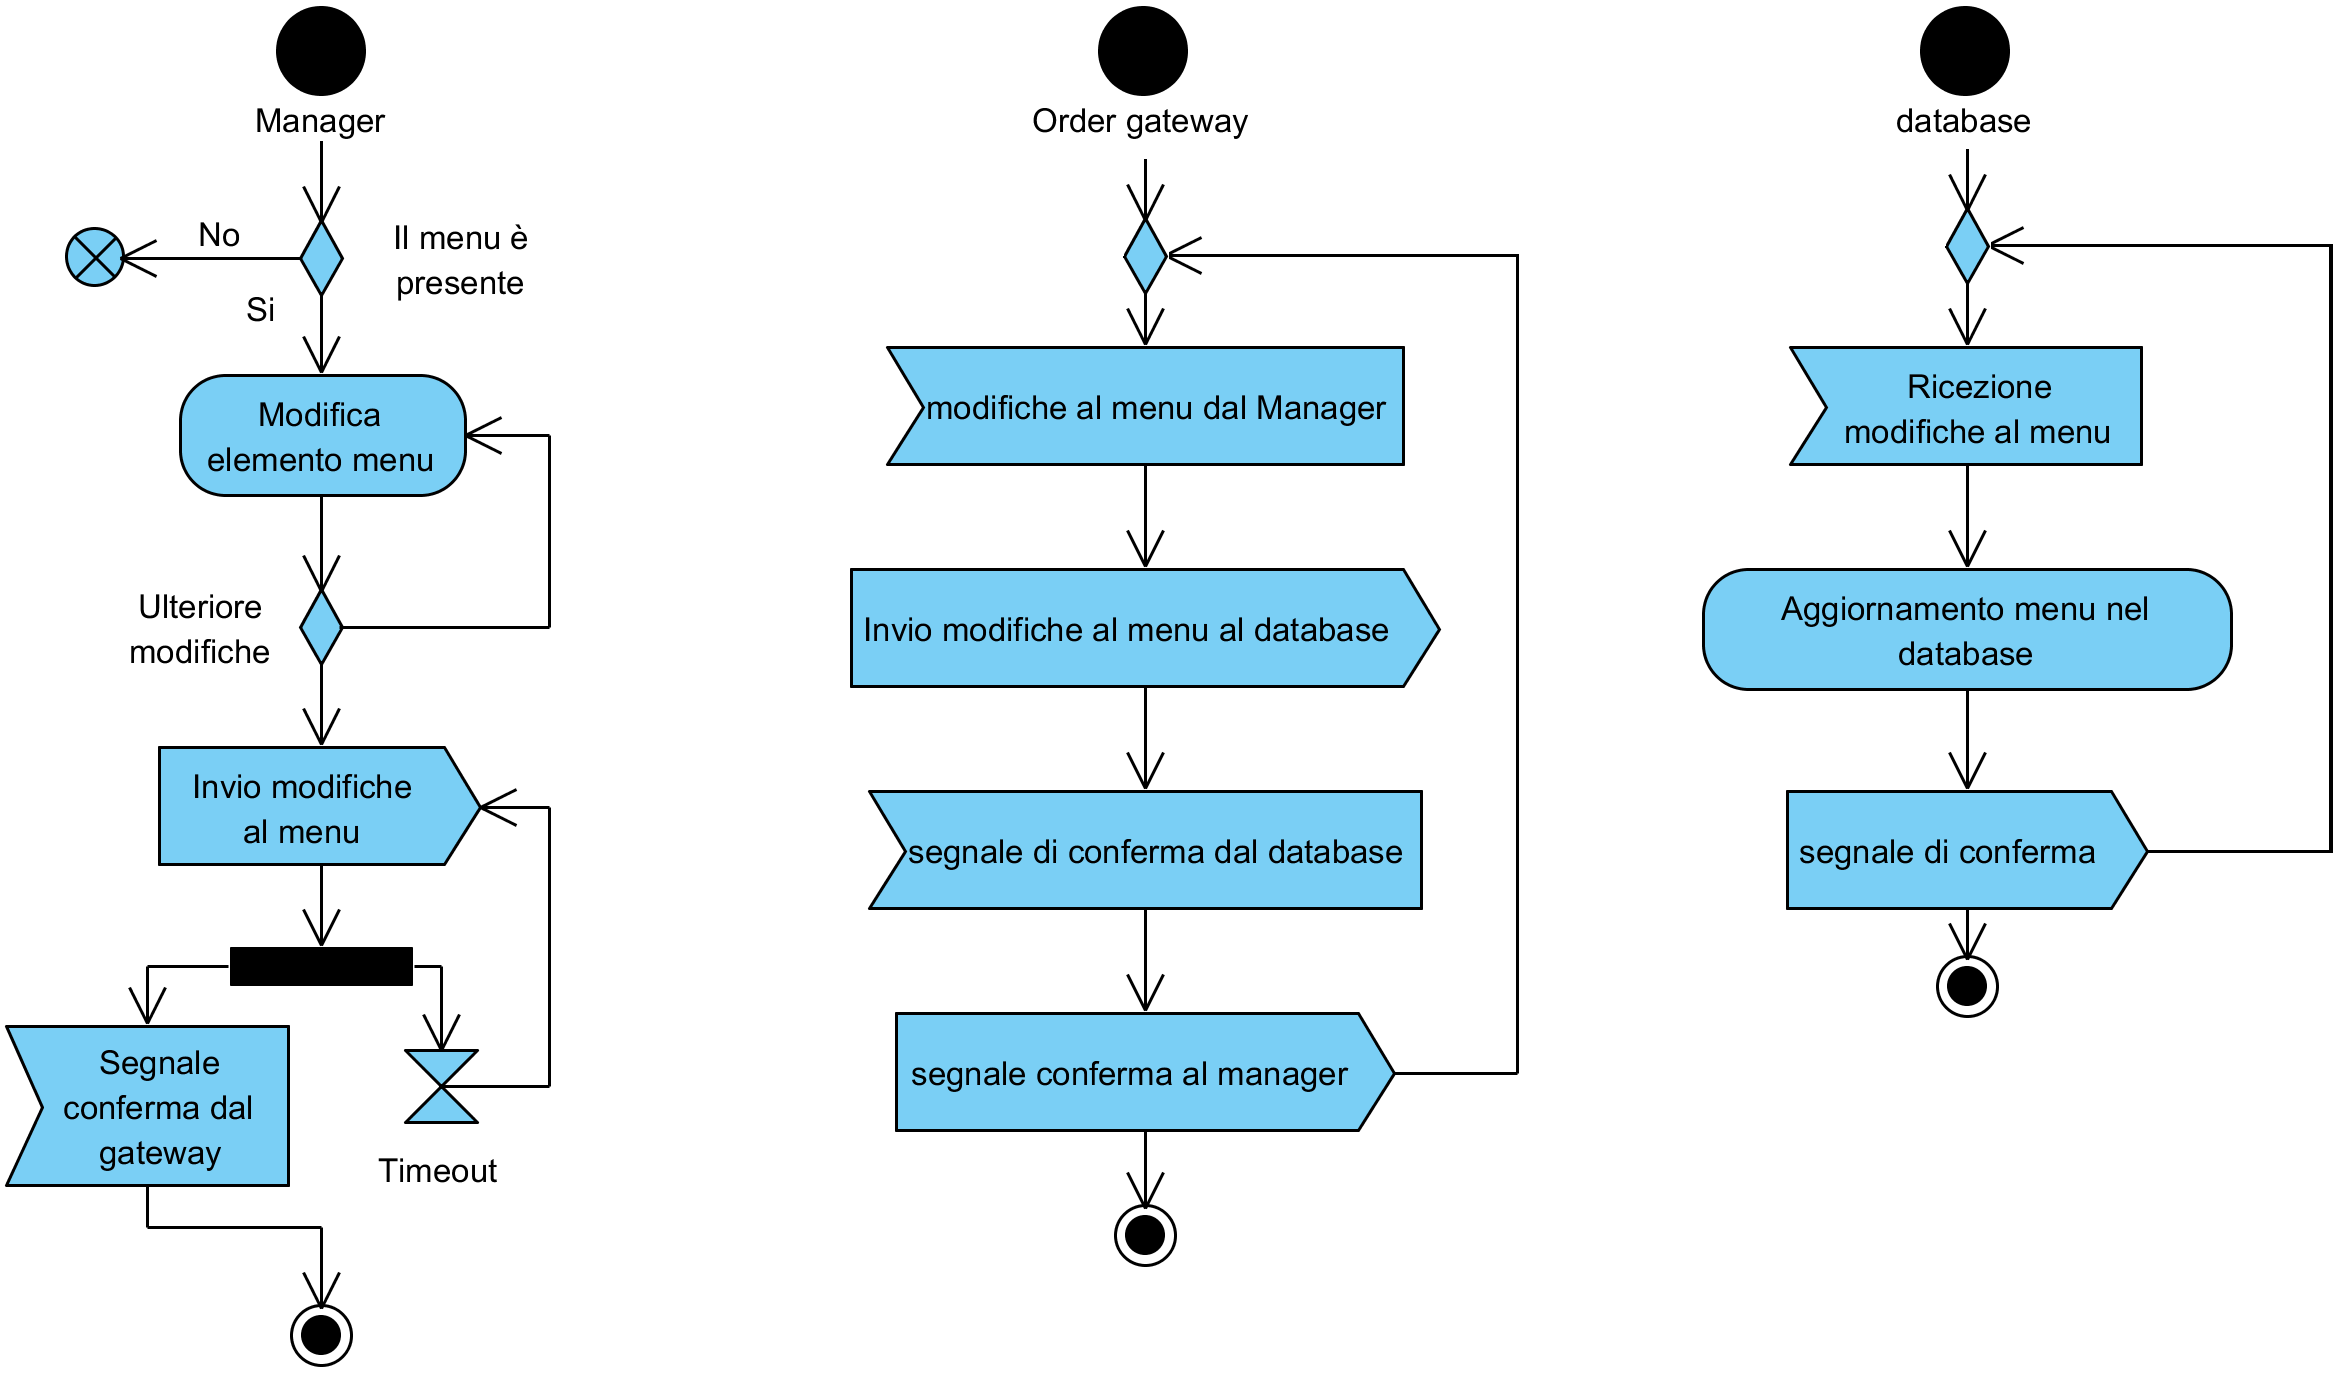
\includegraphics[width=14cm]{diagrammi_img/attivita/manager_menu_modifiche.png}
	\caption{Diagramma di attività - Modifica menu}
\end{figure}

\begin{figure}[H]
	\centering
	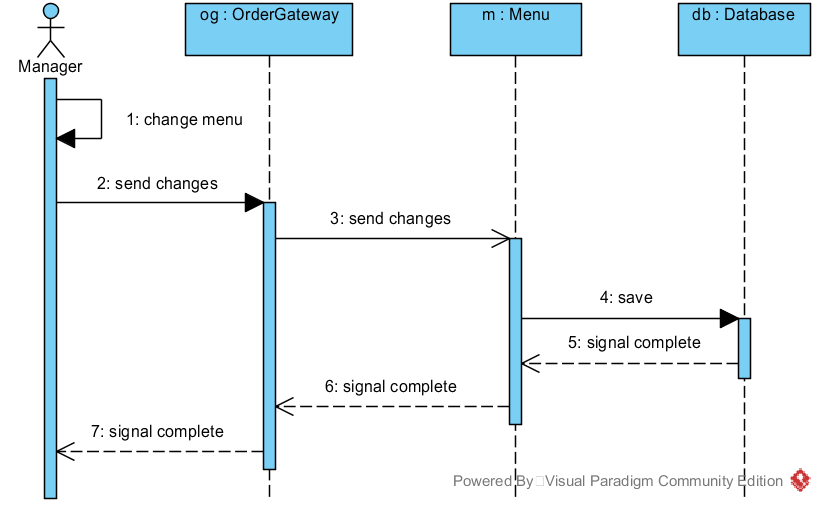
\includegraphics[width=14cm]{../../documenti/SpecificaTecnica/diagrammi_img/sequenza/direttore_modifica_menu.png}
	\caption{Diagramma di sequenza - Modifica menu}
\end{figure}
Il \Manager{}, una volta effettuate le modifiche al menu, le invia all'Order\-Gateway, il quale le inoltra al database. Vengono quindi aggiornate le informazioni sul database e viene ritornato un segnale di conferma, ricevuto e inoltrato dall'Order\-Gateway al \Manager{}.


\paragraph{Visualizzazione magazzino}\mbox{}\\
\nopagebreak
\begin{figure}[H]
	\centering
	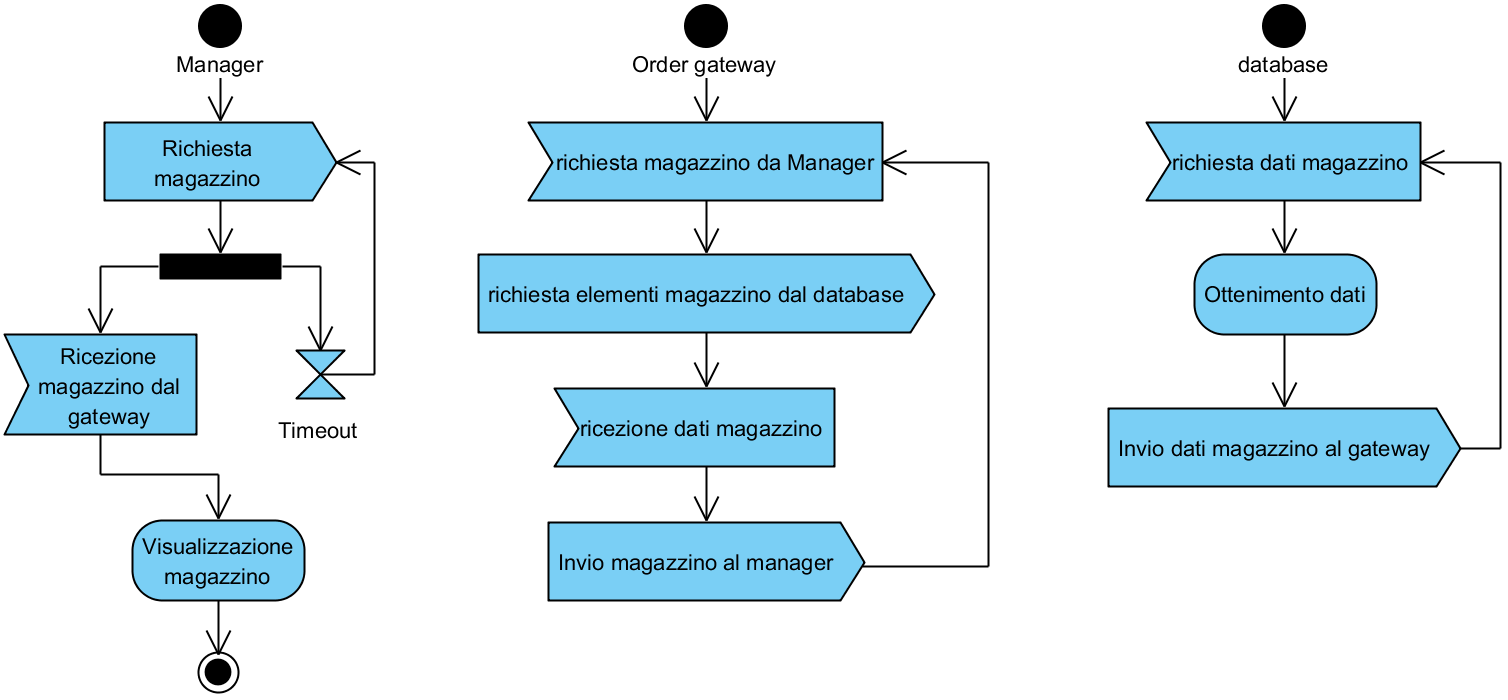
\includegraphics[width=14cm]{diagrammi_img/attivita/manager_mag.png}
	\caption{Diagramma di attività - Visualizzazione magazzino}
\end{figure}

\begin{figure}[H]
	\centering
	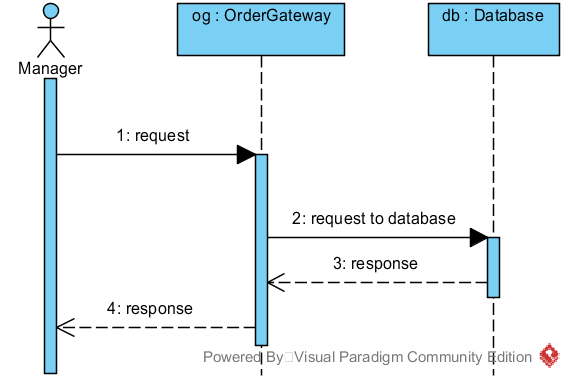
\includegraphics[width=14cm]{../../documenti/SpecificaTecnica/diagrammi_img/sequenza/direttore_visualizza_magazzino.png}
	\caption{Diagramma di sequenza - Visualizzazione magazzino}
\end{figure}
Il \Manager{} effettua una richiesta per visualizzare il magazzino, che viene ricevuta dall'Order\-Gateway e inoltrata al database. Vengono quindi recuperate le informazioni richieste e ritornate all'Order\-Gateway, il quale le inoltra al \Manager{}.

\paragraph{Modifica magazzino}\mbox{}\\
\nopagebreak
\begin{figure}[H]
	\centering
	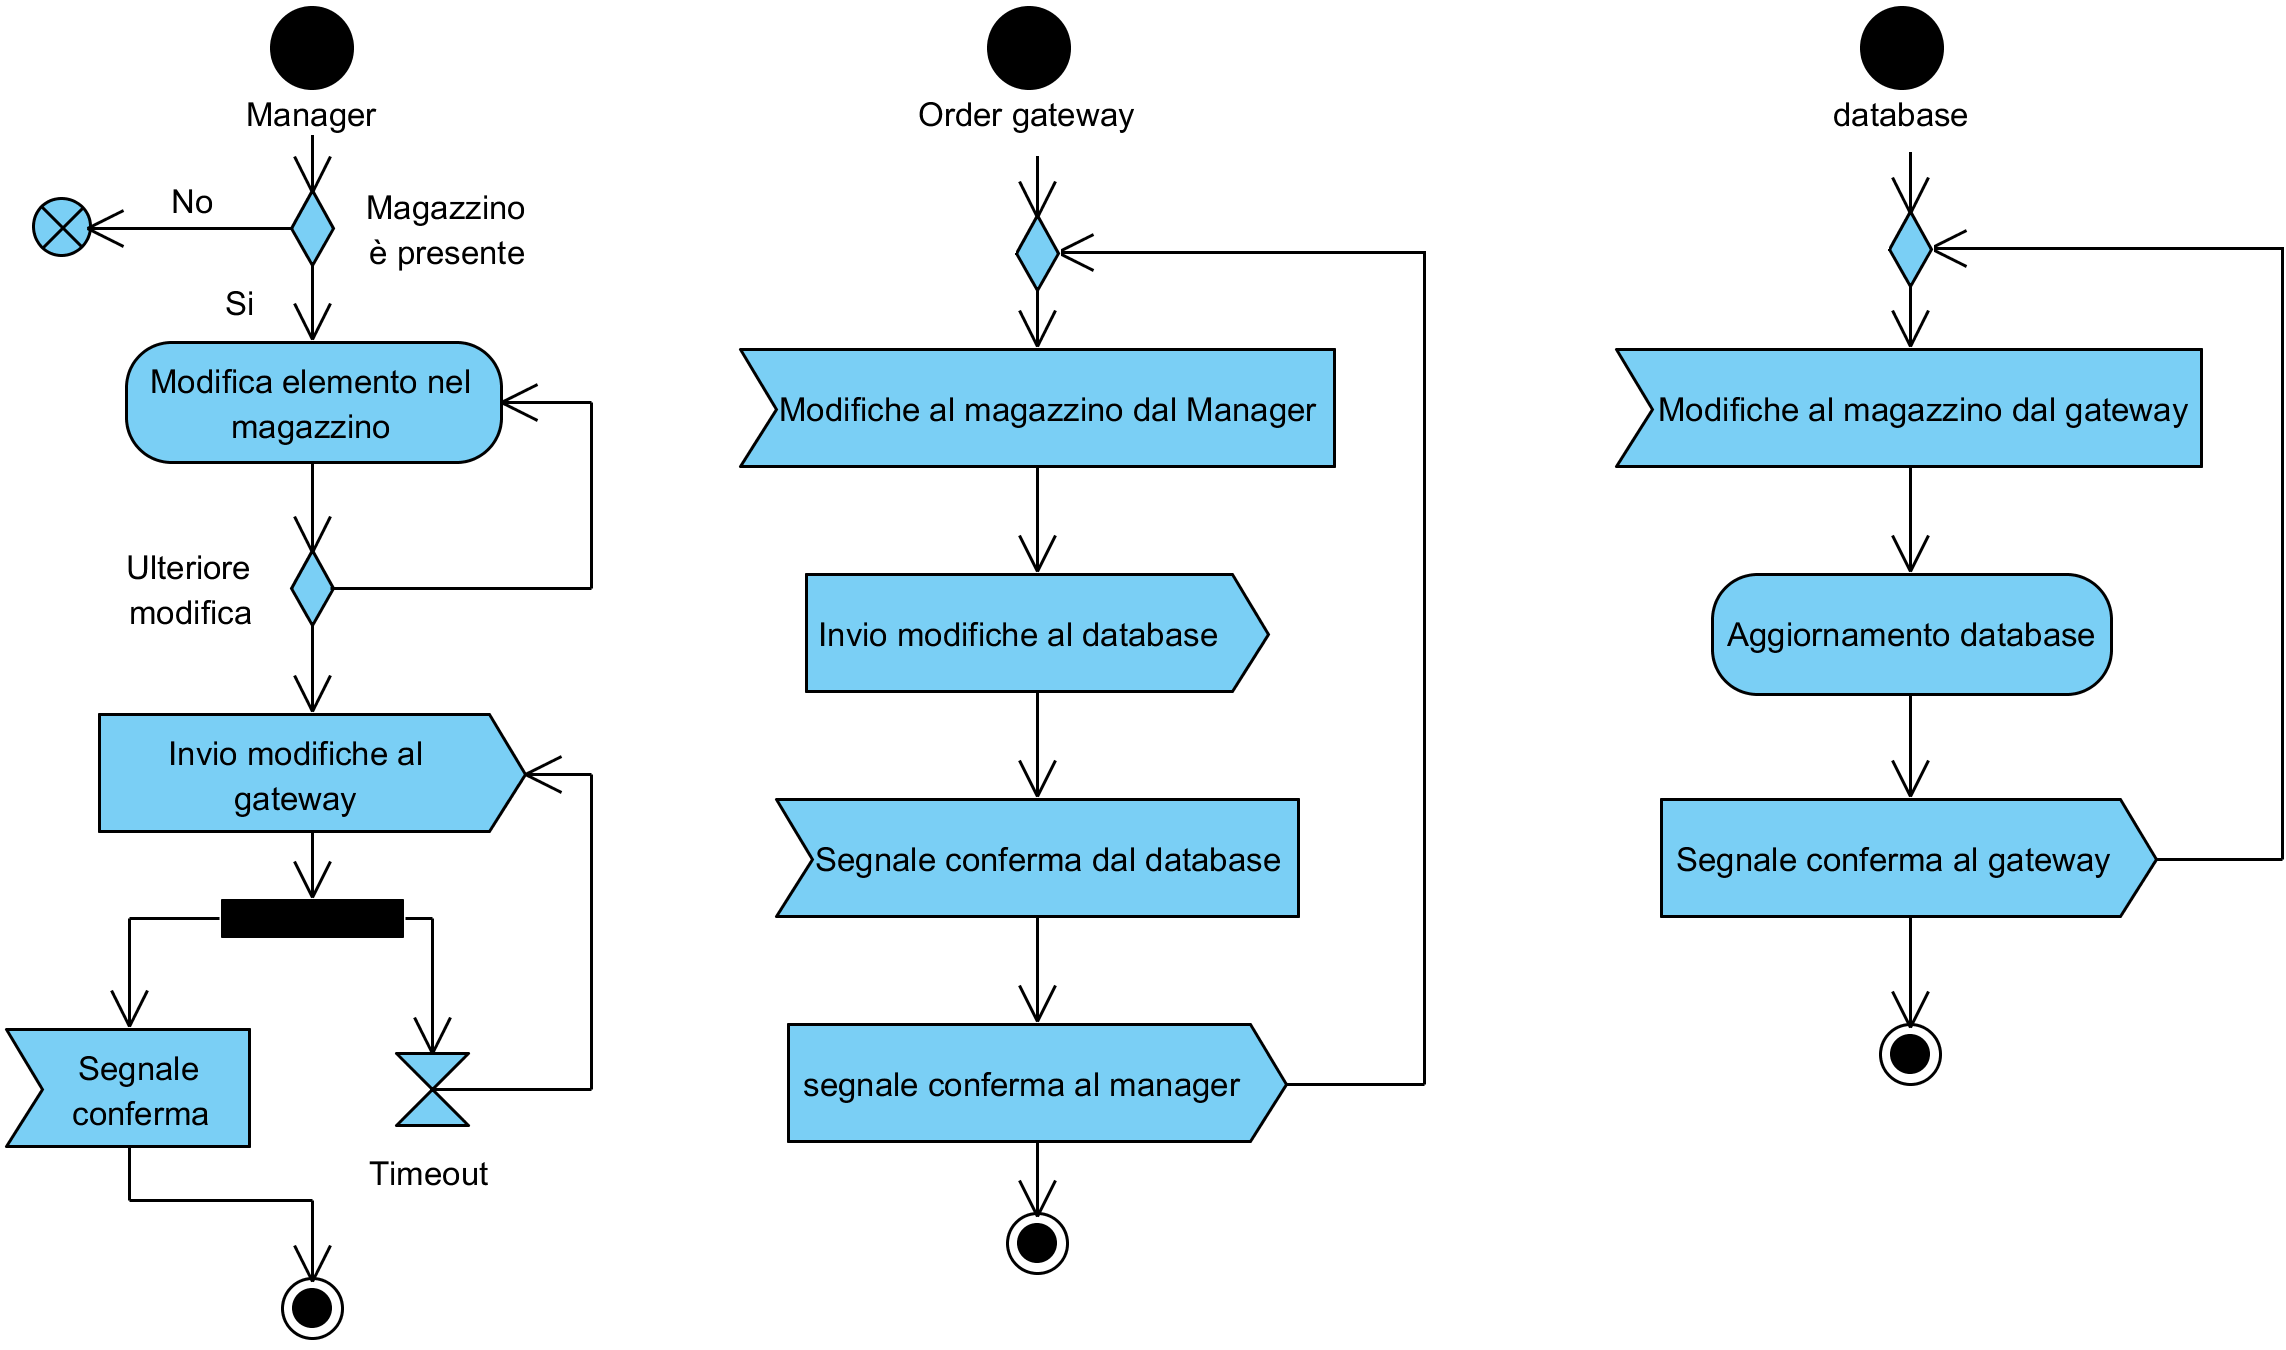
\includegraphics[width=14cm]{diagrammi_img/attivita/manager_mag_modifiche.png}
	\caption{Diagramma di attività - Modifica magazzino}
\end{figure}

\begin{figure}[H]
	\centering
	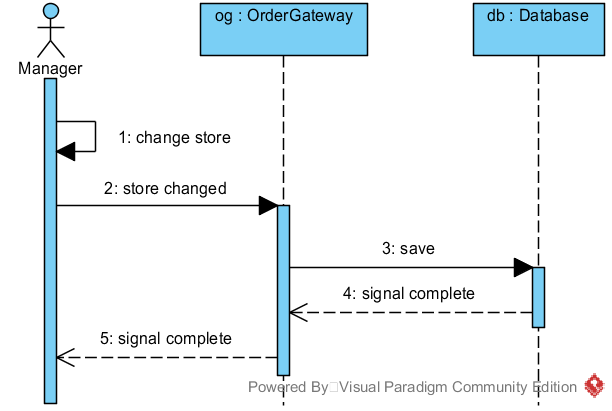
\includegraphics[width=14cm]{../../documenti/SpecificaTecnica/diagrammi_img/sequenza/direttore_modifica_magazzino.png}
	\caption{Diagramma di sequenza - Modifica magazzino}
\end{figure}
Il \Manager{}, una volta effettuate le modifiche al magazzino, le invia all'Order\-Gateway, il quale le inoltra al database, che provvede ad aggiornare i dati. Il database ritorna quindi un segnale di conferma all'Order\-Gateway, che lo inoltra al \Manager{}.


\paragraph{Visualizzazione orders}\mbox{}\\
\nopagebreak
\begin{figure}[H]
	\centering
	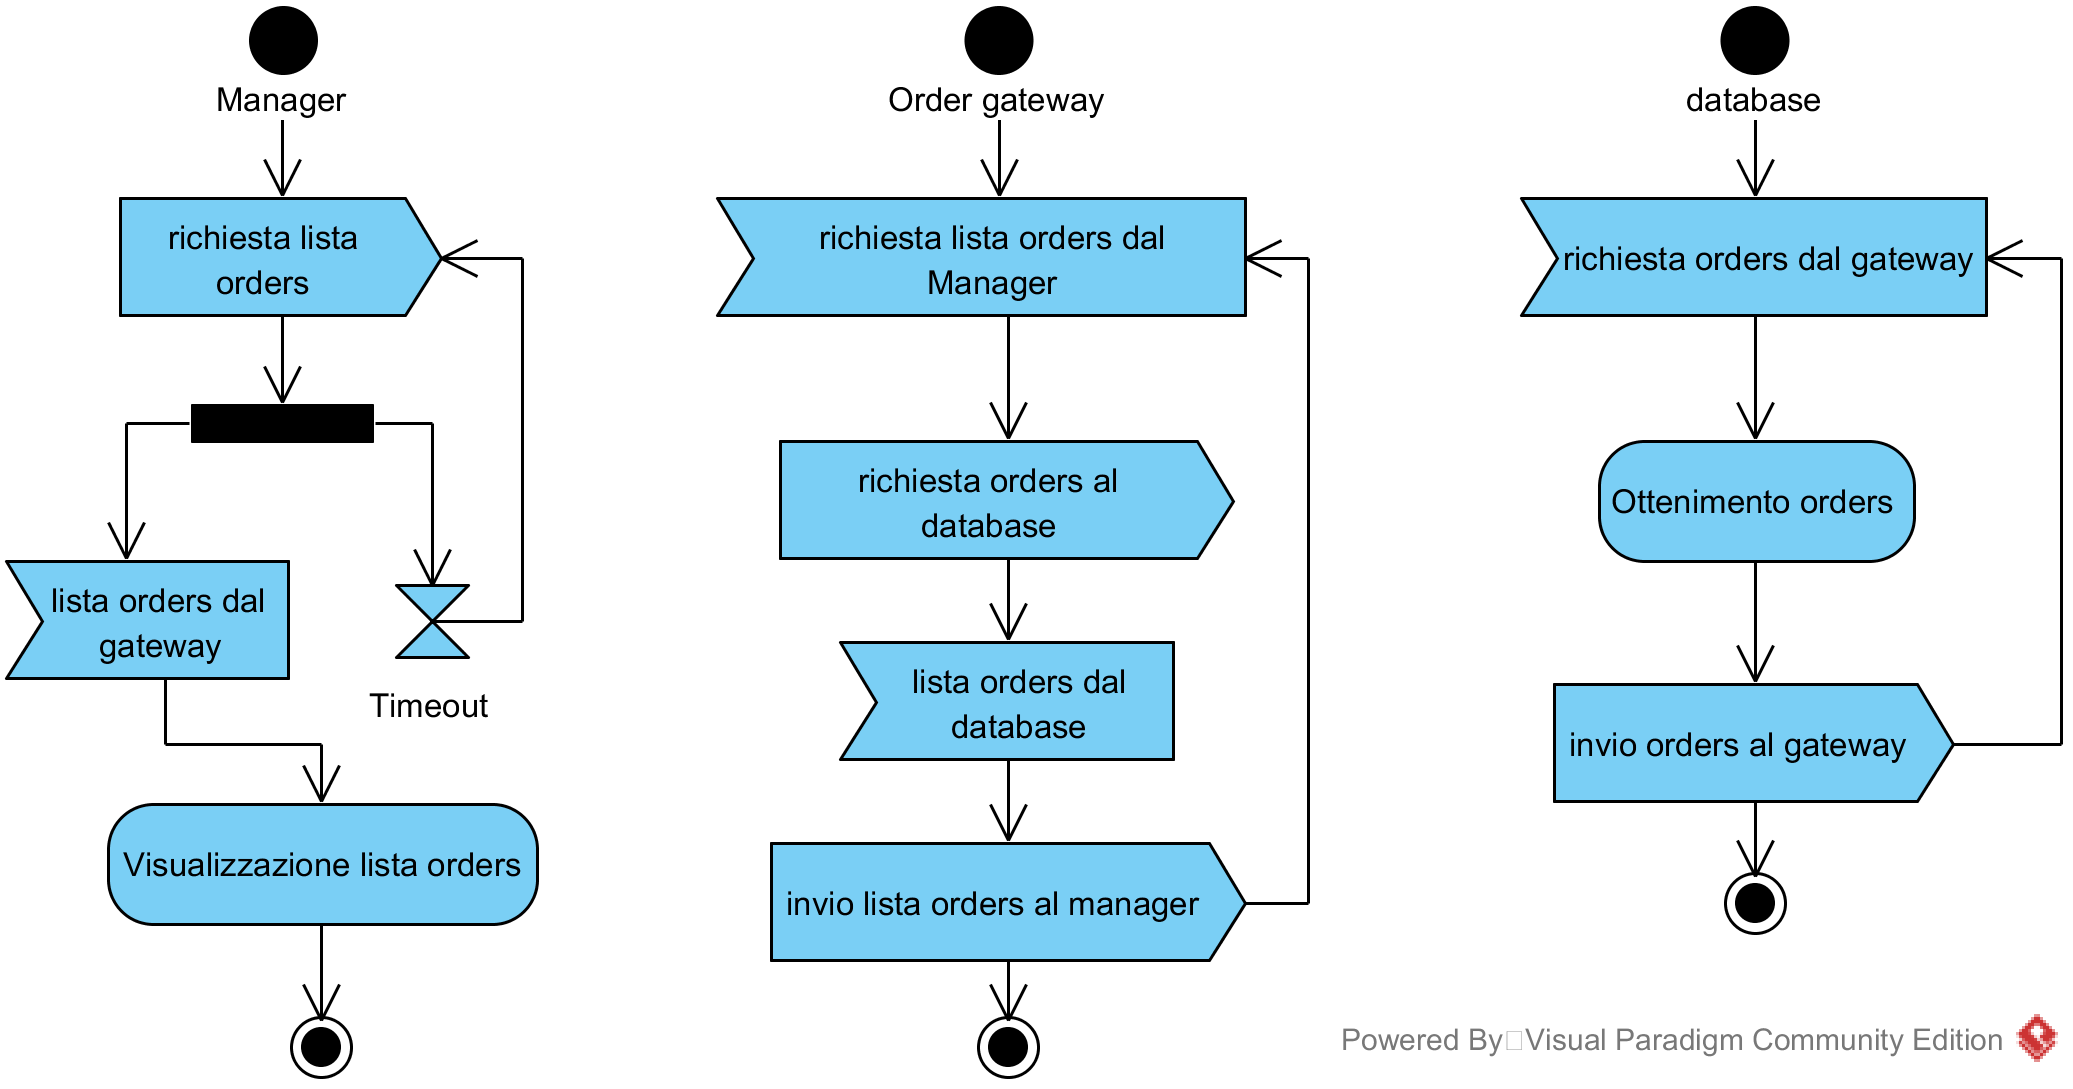
\includegraphics[width=14cm]{diagrammi_img/attivita/manager_ordini.png}
	\caption{Diagramma di attività - Visualizzazione orders}
\end{figure}

\begin{figure}[H]
	\centering
	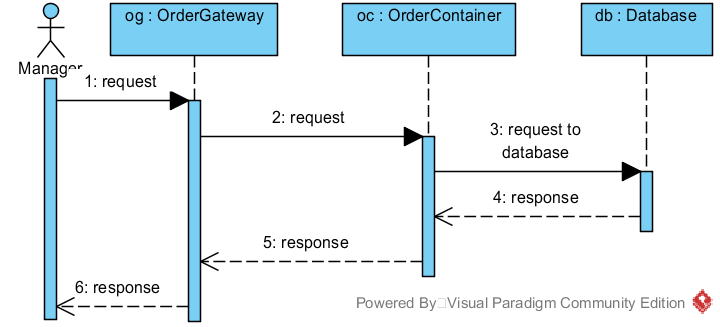
\includegraphics[width=14cm]{../../documenti/SpecificaTecnica/diagrammi_img/sequenza/direttore_visualizza_orders.png}
	\caption{Diagramma di sequenza - Visualizzazione orders}
\end{figure}
Il \Manager{} effettua una richiesta per visualizzare gli ordini all'Order\-Gateway, il quale la inoltra al database. Vengono quindi recuperati gli ordini di interesse, restituiti in risposta dal database all'Order\-Gateway, il quale a sua volta inoltra i dati al \Manager{}.

\paragraph{Elimina orders}\mbox{}\\
\nopagebreak
\begin{figure}[H]
	\centering
	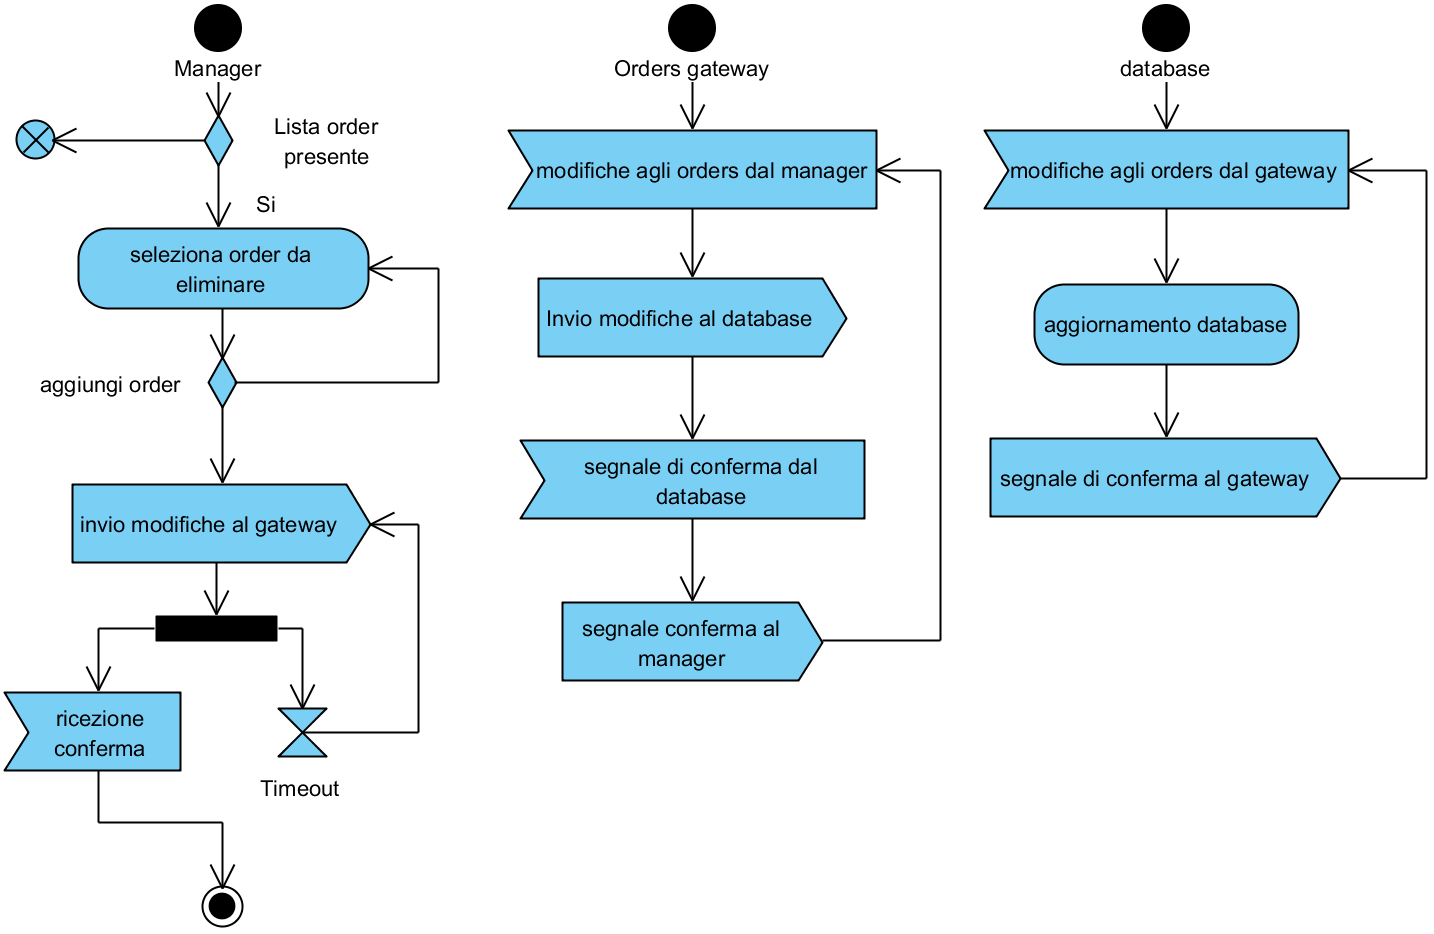
\includegraphics[width=14cm]{diagrammi_img/attivita/manager_order_remove.png}
	\caption{Diagramma di attività - Elimina order}
\end{figure}

\begin{figure}[H]
	\centering
	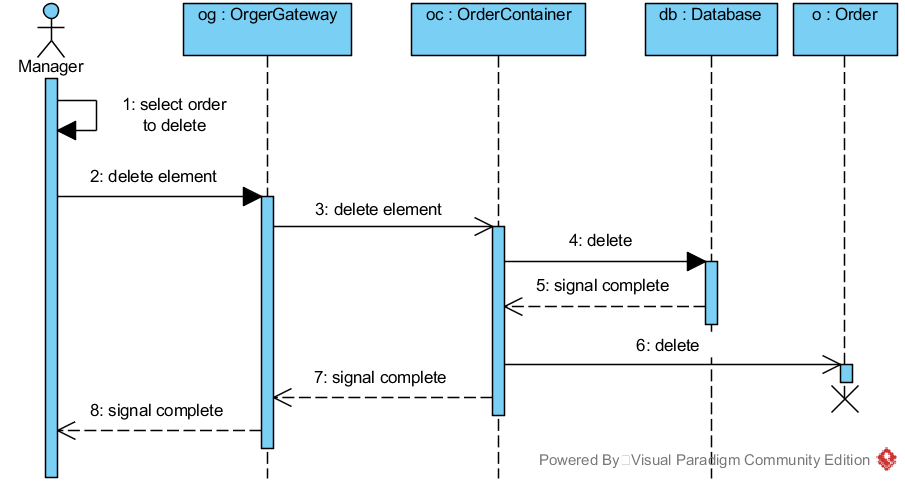
\includegraphics[width=14cm]{diagrammi_img/sequenza/direttore_elimina_orders.png}
	\caption{Diagramma di sequenza - Elimina order}
\end{figure}
Il \Manager{} seleziona dagli ordini da eliminare ed invia la richiesta all'Order\-Gateway, il quale la inoltra al database. Vengono quindi eliminati gli ordini selezionati e viene inviato un segnale di conferma dal database all'Order\-Gateway, il quale a sua volta lo inoltra al \Manager{}.
